\normalsize
\begin{FlushLeft}
    \section{Technical Design}

    \subsection{Programming Language Selection and Libraries Used}

    I selected C# as my programming language for several reasons. Currently, it is the language that I am most familiar with. In addition, I conducted research on which languages are best for fast processing, and found that C, C++, and C# are among the top contenders. Considering my skill set and the importance of speed in this situation, I concluded that C# would be a good fit. Furthermore the object orientated nature of the language means that I will be able to separate the front end and the back end processing into separate bll files keeping the code clean and easily maintainable.\\ 
    \bk
    Find below a list of all libraries I used: \\
    
    \subsubsection{Linq}
    In order to manipulate lists and create the data structures that I need I will need to use some Linq methods. During the prototyping stage I found that using some Linq methods such as the Select statement allowed the program to be easier to read and make logical sense. As well as this there have been optimisations made in the iterative Linq methods which will make my program faster. Similar to some of the following libraries this is a Microsoft Library which is open source.
    \\ \bk


    \subsubsection{Bitmap}
    In order for my program to function a required part of it is that it is able to take an image as an input. In native C# there is no set way to do this. Therefore I needed to use the Microsoft System.Drawing Namespace. This namespace provides access to GDI+ basic graphics functionality. This does limit this project as is to only working on Windows since the library requires access to the GDI+ native library which is only on windows services. \\
    
    The only part of this library I will be using is the Bitmap class. This will allow me to accept all types of images without the need of parsing them myself since this is not the aim of my project. 
    \\ \bk

    \subsubsection{Windows Forms}
    In order to complete my objectives my program will need to be easy to use and any user with some degree of technical competency should be able to use it. In order to achieve this objective I though that instead of using some form of console input in order to get a starting and an end location, that it would be better to use some form of GUI. In order to do this I will use Windows Forms. This will allow me to make a simple GUI which will allow the end user to interact with the user and easily understand. \\ 

    The things which I will end up using the windows forms are the map traversal, allowing the user to select a start and an end node with a click instead of having to enter a coordinate. As well as this I will also use forms to show the user the stages of, for example, the Canny edge detection.
    \\ \bk

    \subsection{High Level Overview}
    The general purpose of my project is to allow a user to take a map and input it into my program, then subsequently convert it into a routable map. \\ \bk
    
    In order to achieve this goal my program will first take an input, the users map. It will then take this map and convert it into an machine readable format, a Bitmap. Canny edge detection will then be performed on it causing the edges and the surroundings of the paths on the image to be found. Using these edges a filling algorithm will fill the spaces encapsulated by the lines. Finally these filled spaces will be used to convert the whole image to a graph which can then be traversed using graph traversal algorithms such as A* or Dijkstra's algorithm. \\ \bk

    \begin{figure}[H]
        \centering
        \subfloat[\centering Data Flow Diagram]{{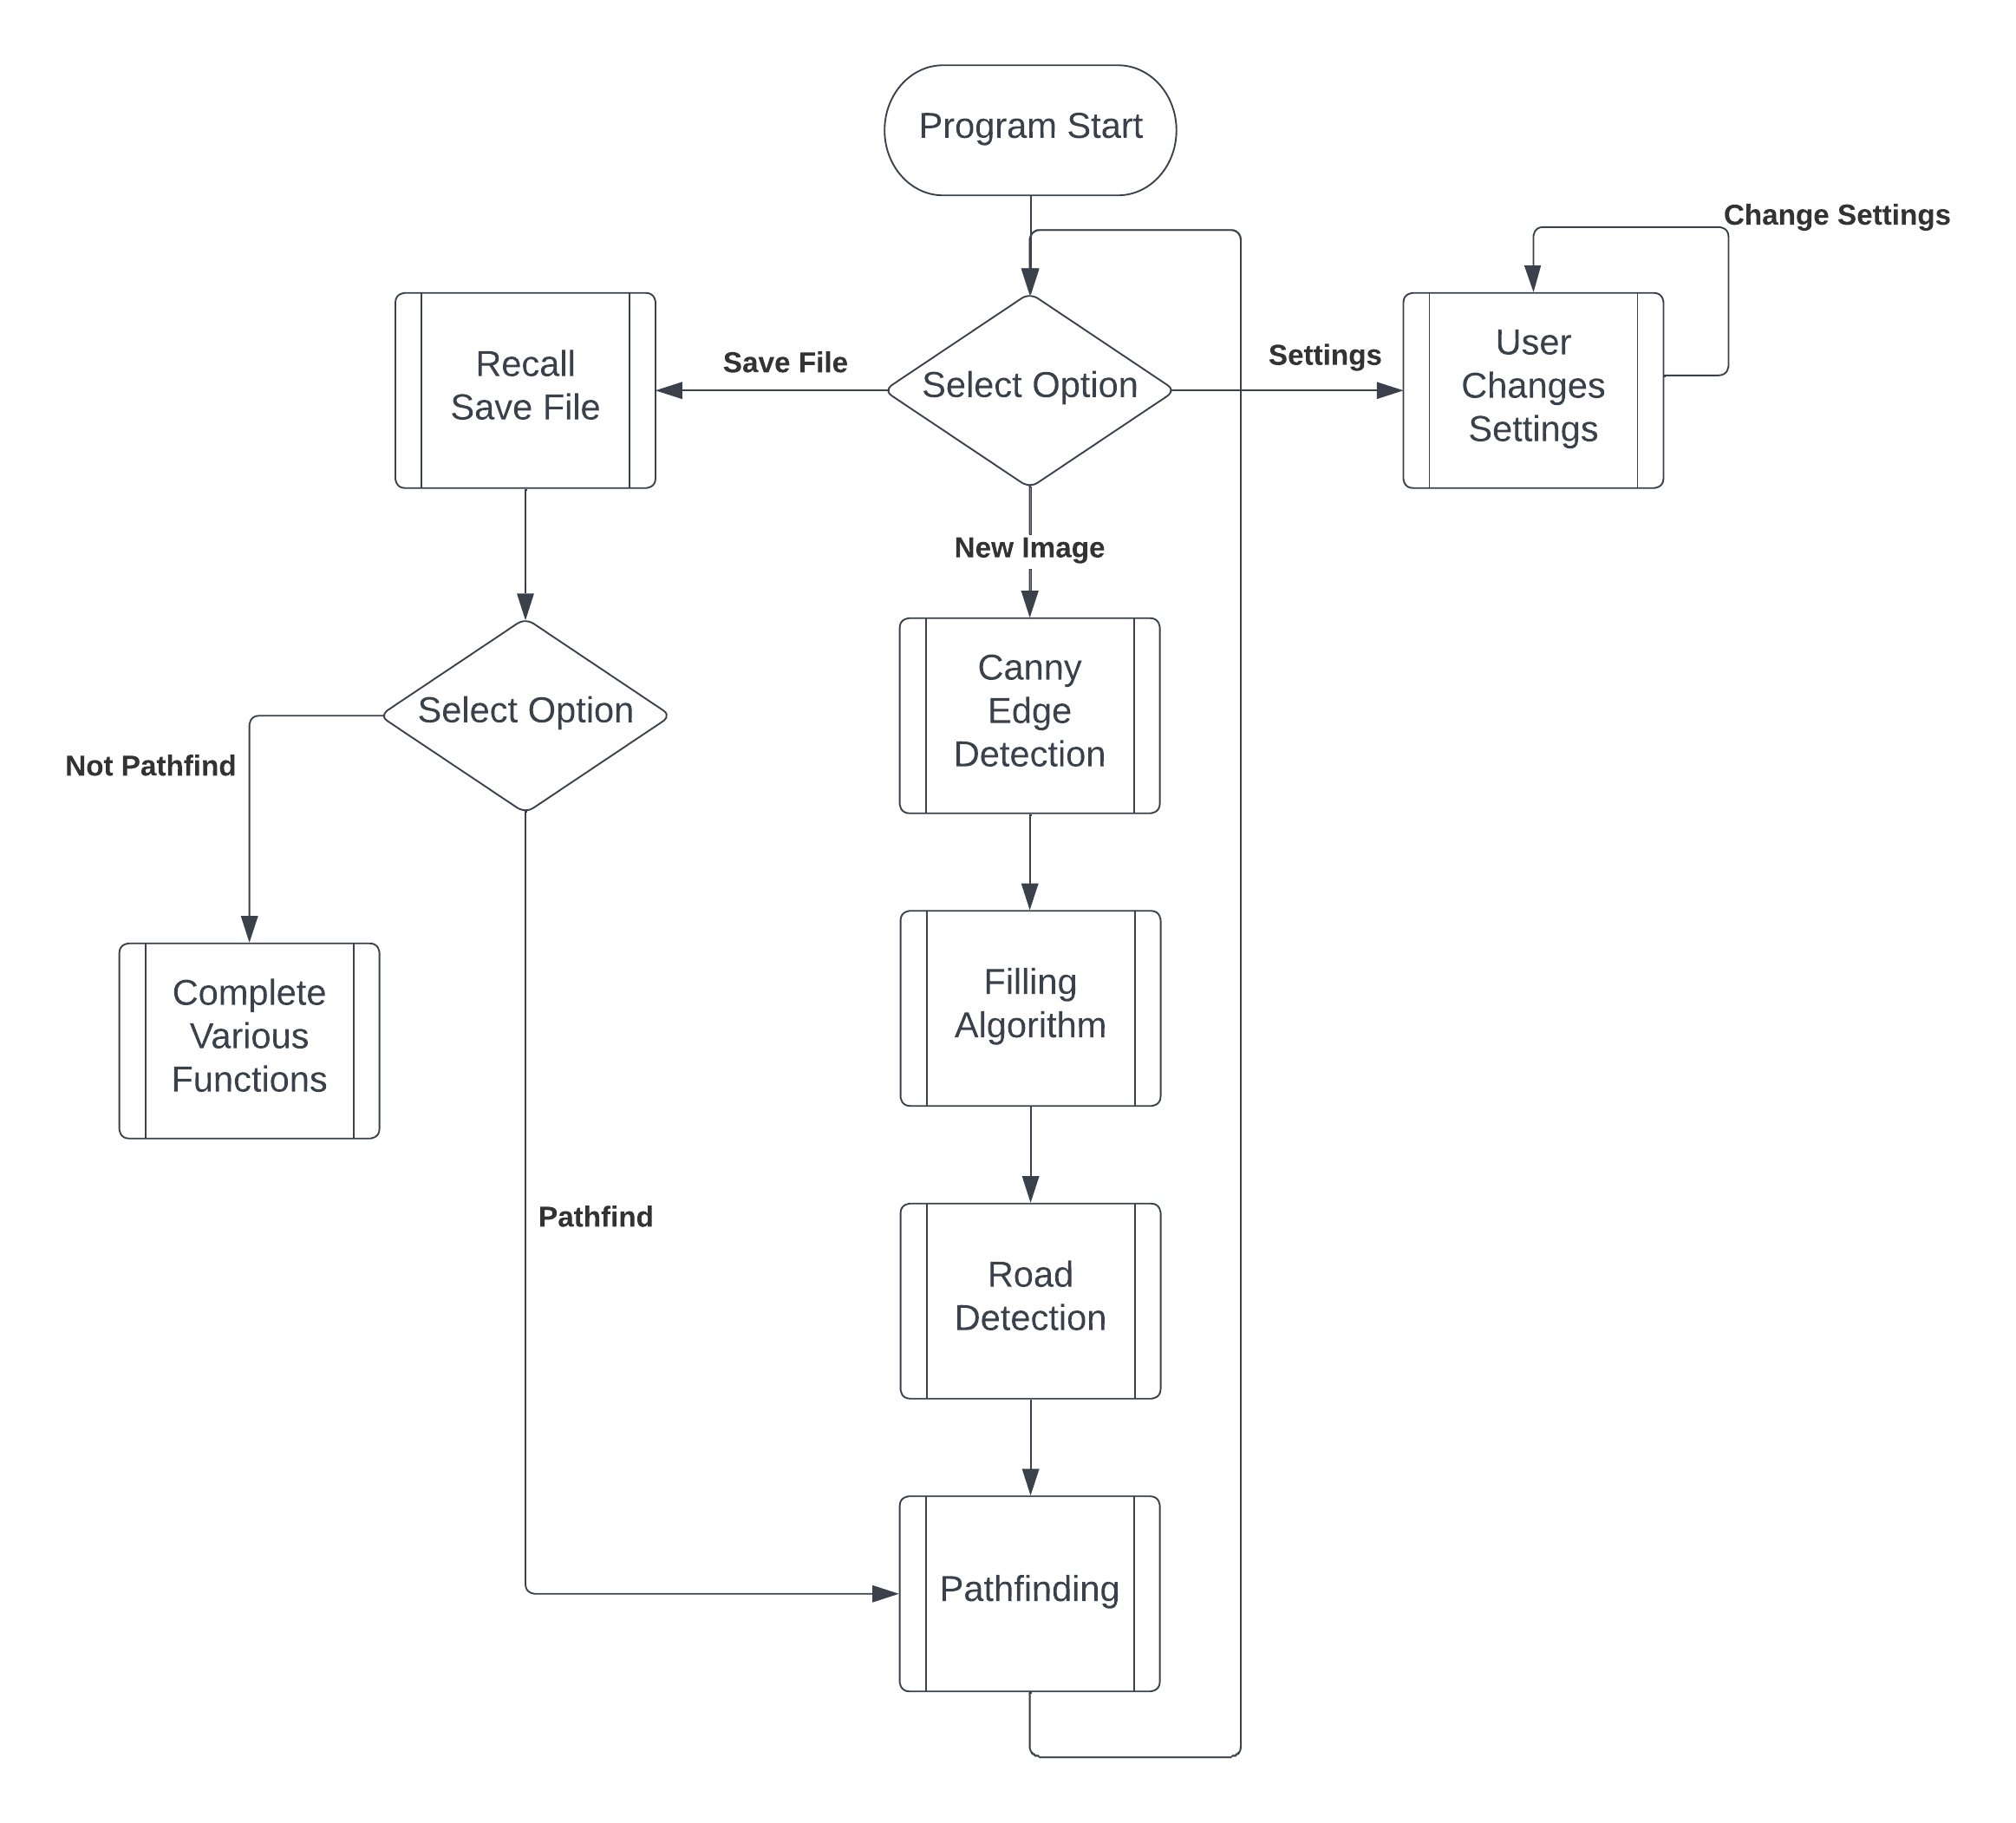
\includegraphics[width=17.2cm]{images/HighLevelOverview.png}}}
    \end{figure}

    This is a high level overview of the flow of data through the program, find a more detailed one below.\\ \bk

    The version of Edge Detection I will be using as previously stated will be Canny Edge Detection, this is as opposed to Sobel Edge Detection. The main version of filling I will be using is flood fill due to it simple nature to implement ad due to the fact that it does not take much memory and can be made recursive so it performs well. The final main algorithm I will need to use is image kernels and convolution, this will allow me to manipulate the inputted image.

    \subsubsection{Full DFD (Data Flow Diagram)}
    \begin{figure}[H]
        \centering
        \subfloat[\centering Full DFD]{{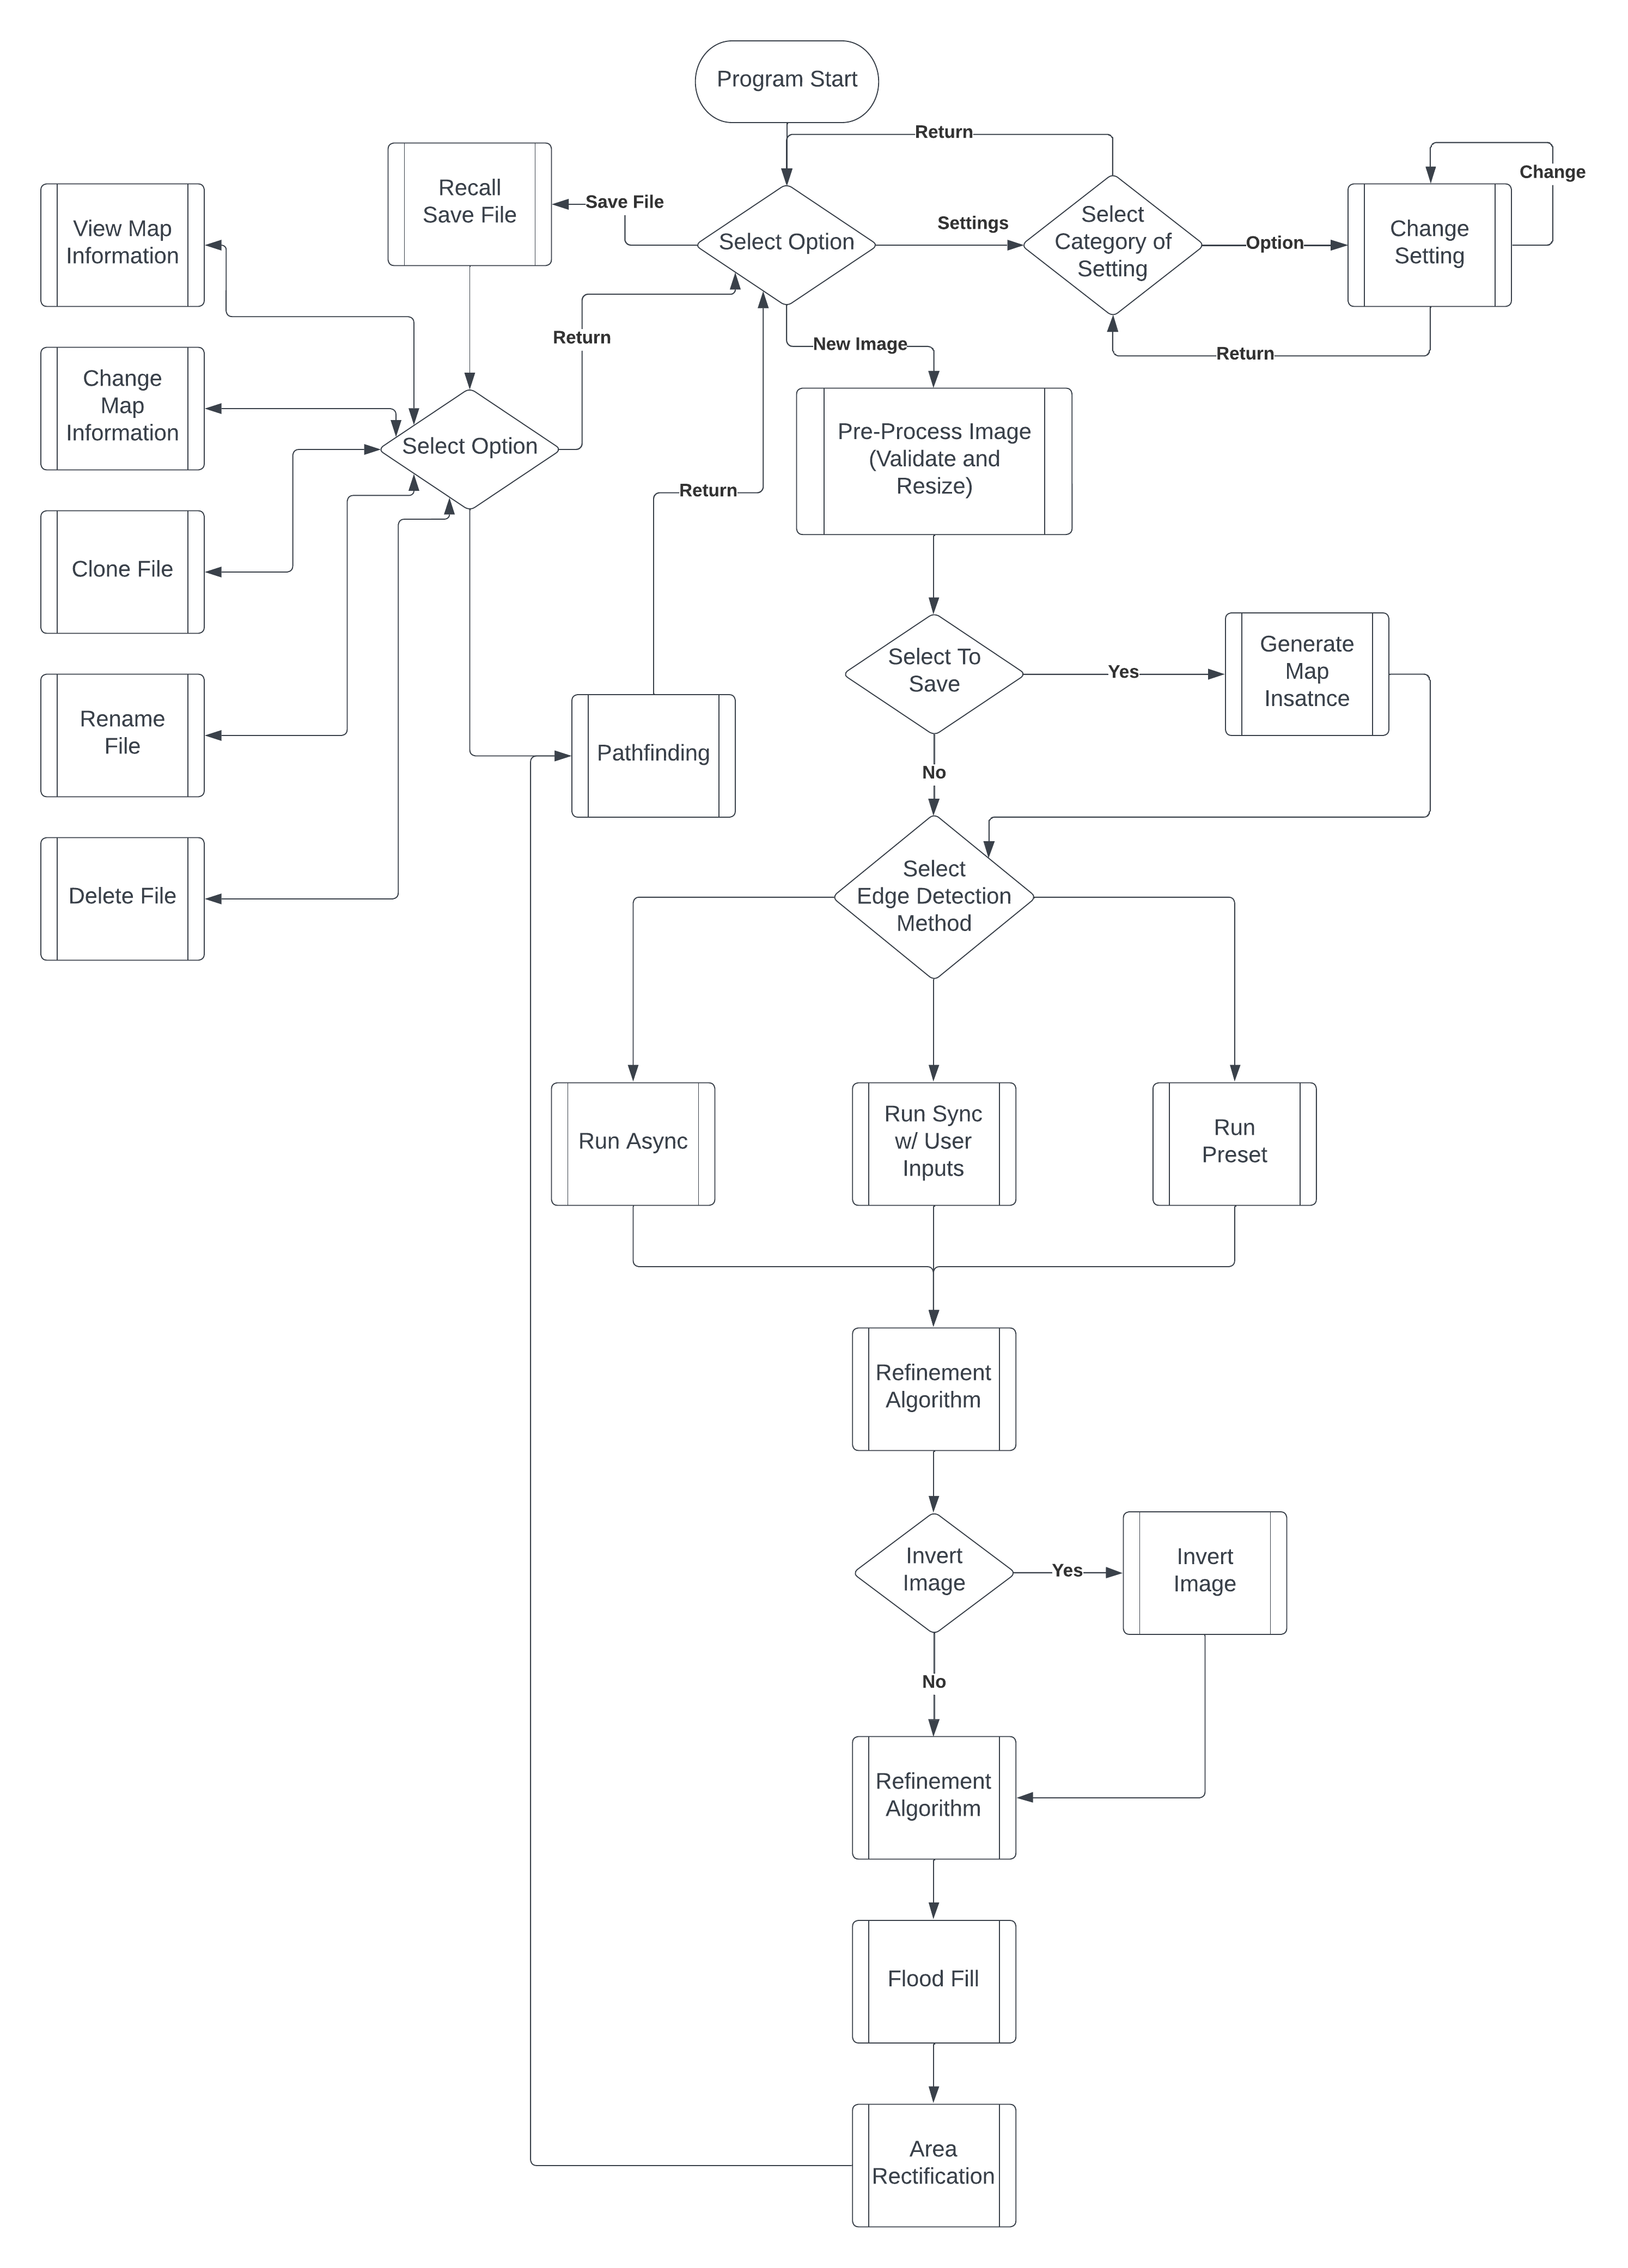
\includegraphics[width=16cm]{images/FullDFD.png}}}
    \end{figure}

    \subsubsection{Backend Library}
    For my project to ensure that I conform to the OOP principle of encapsulate what varies. I will accomplish this through the use of classes and encapsulation. Furthermore I have also made the decision to split up my solution into two separate projects, this means that my program will produce two files in order to run, one of these will be the DLL for the backend library and the other will be the executable for the front end. \\ \bk

    Contained within this backend section of my program will be contained the edge detection, road detection, complex data types and graph traversal algorithms as well as various utilities that are frequently used throughout the program. \\ \bk

    One of the main features of the backend library are the custom structures that have been created in order to allow for easier processing of data. Find below the image of the structure class layout and the classes which link within.\\

    \begin{figure}[H]
        \centering
        \subfloat[\centering Overview of Backend Structures]{{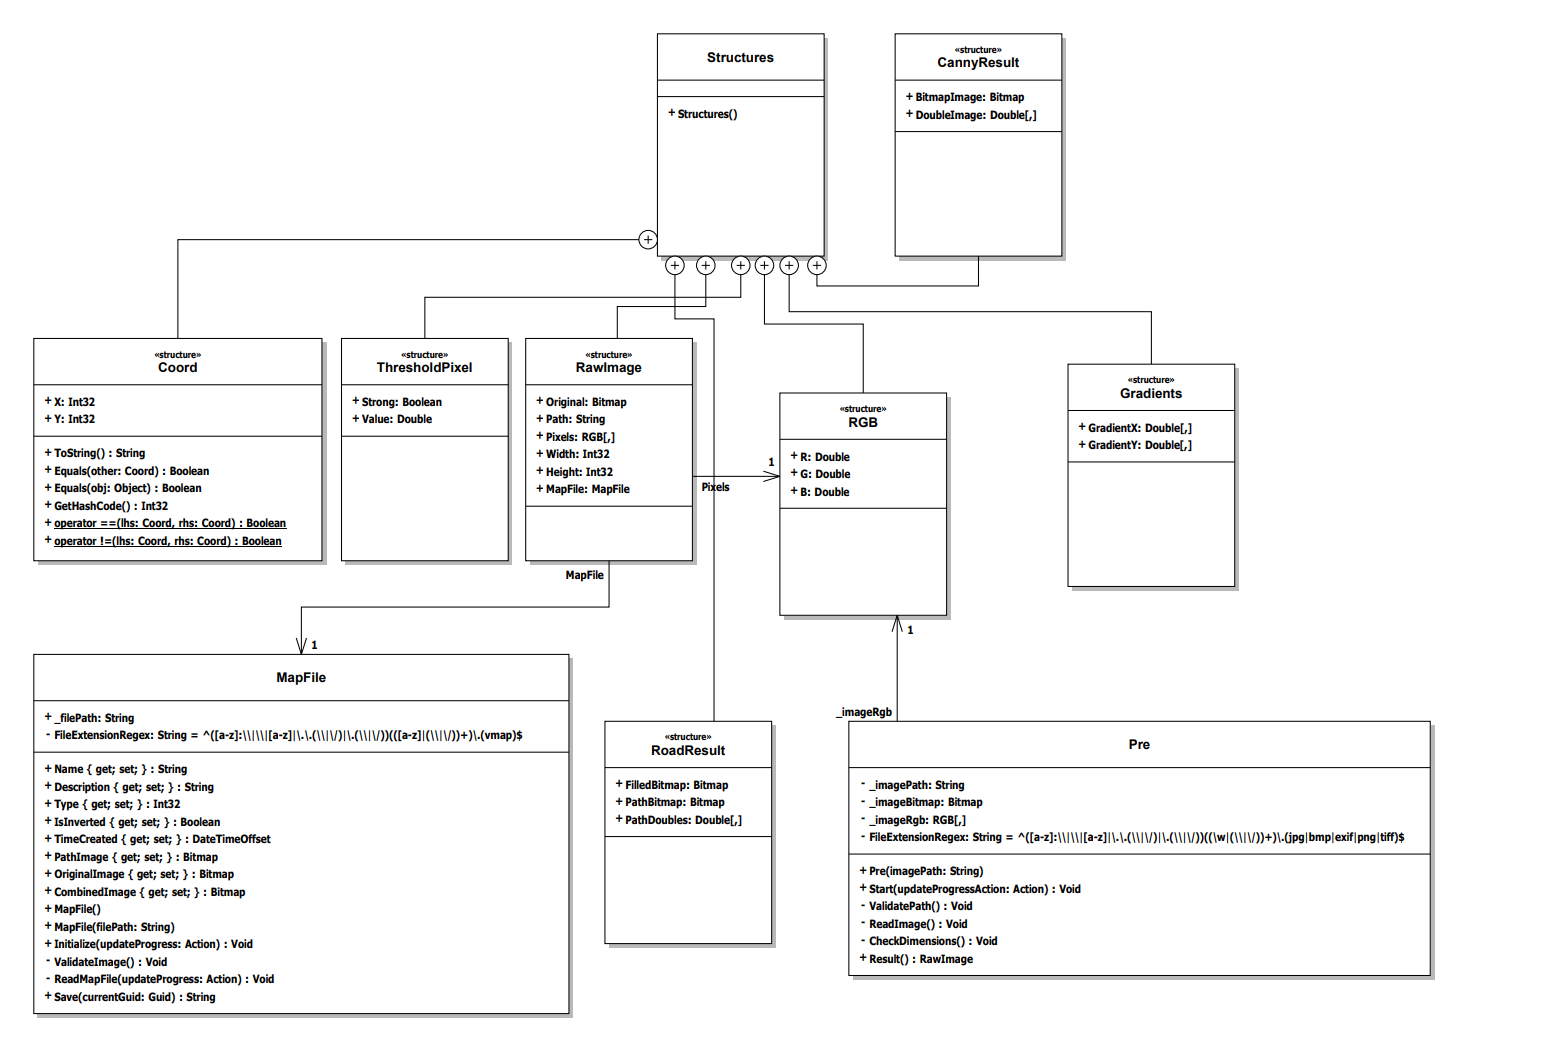
\includegraphics[width=17.2cm]{images/UML/Backend.png}}}
    \end{figure}

    \\

    As can be seen form the class diagram of the backend library, there is very little dependency within the library itself. This allows the backend to function independently of the program which is using it. This allows the backend to be split out and moved to another program if needed. Summarised there are four main reasons to do this:

    \begin{itemize}
        \item \textbf{Modularity} - By separating the backend from the frontend one is able to be built without the other. This means that when working on my project I can take time to perfect one without impacting the other.
        \item \textbf{Reusability} - As previously stated being able to be reused is a large reason as to why to separating the elements is a good idea. Since if I wanted to expand this project for example and make a web interface for it, I could take the maths of the backend and recreate the front end in a web framework like Razor Pages.
        \item \textbf{Maintainability} - It is allot easier to maintain code when it has been organised into classes and by extension into libraries where a library is a collection of classes. It means that should something throw an error in the backend I would be able to easily isolate the issue and be able to fix it.
        \item \textbf{Testability} - In a similar vain to the Maintainability of the program being modular also means that it is very easy to implement testing. This means that as I go thorough making my program it will make it allot easier to separate variables and make isolated testing conditions. Furthermore it means that I can test the maths of the Canny Detection without having to worry about making an interface to it using the UI.
    \end{itemize}
    \\ \BK

    \subsubsection{Local Application}
    The local application part of this program will be responsible for the tying if the various algorithms of the backend together along with providing the user with a way to interact with them, whether this is through the use of windows forms of the console for text inputs. As stated by objective 5 the design of the UI should be simplistic and easy to understand at a glance, therefore I will only be using the methods as stated above for interacting with the user. I also believe that it will be best to keep the changes between the two to a minimum and when there is a change make sure that the user is aware of it before hand.\\ \bk
    
    \paragraph{Design of User Interface (Console)} \mbox{} \\
    In order to keep the user interface as easy to use as possible the console will remain static while the program is being run. This means that once it has been started and set to its correct size it will form itself to fit the screen and will only run if it has been maximized. This will allow me to make sure that the interface is clear and easy to use. Find below a mock-up of the console design.
    
    \begin{figure}[H]
        \centering
        \subfloat[\centering Mock-up of Console Interface]{{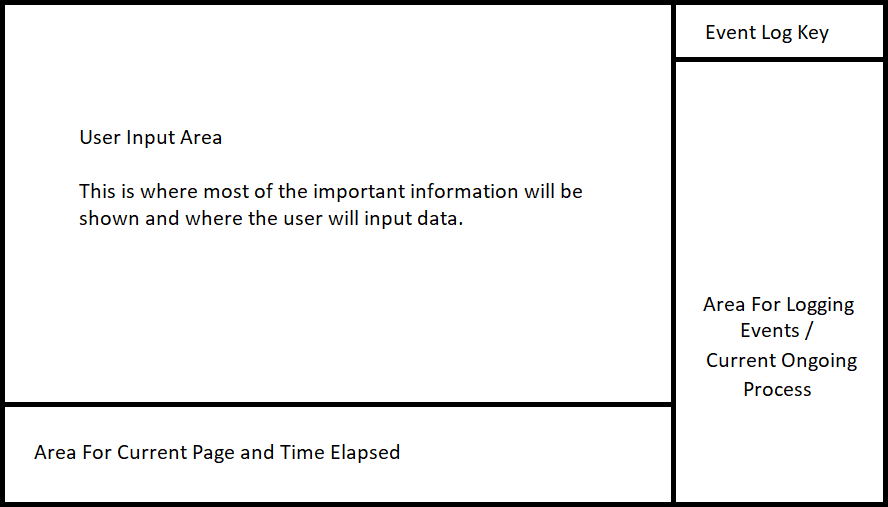
\includegraphics[width=12.5cm]{images/design/consoleMock.png}}}
    \end{figure}\\

    As can be seen in this mock-up fo the console interface it can be seen that there is a large section for the user to enter and view important in. As will be expanded on in the second section about the Windows Forms interface, due to the static nature of the console I will be able to make a Form conform to the shape of this area. See the next paragraph for more information. \\ \bk

    As for the other elements of the console UI, as part of objective 5, this must be easy to see at a glance what is going on and which step you are in. To accomplish this on the right hand side of the console there will be a log which, should the user select to do so in settings, will display each method call and the result of that call allowing them to see exactly where they are in the process. \\ \bk
    
    At the bottom of the console in the section labelled "Area for Current Page and Time Elapsed" this will be used for, as the name suggests, the current page and time elapsed. What this means is that at a glance a non-technical user or one who has opted not to have the advanced logging will still be able to see where they area at in the current process. \\ \bk

    \begin{figure}[H]
        \centering
        \subfloat[\centering Mock-up of Console Interface]{{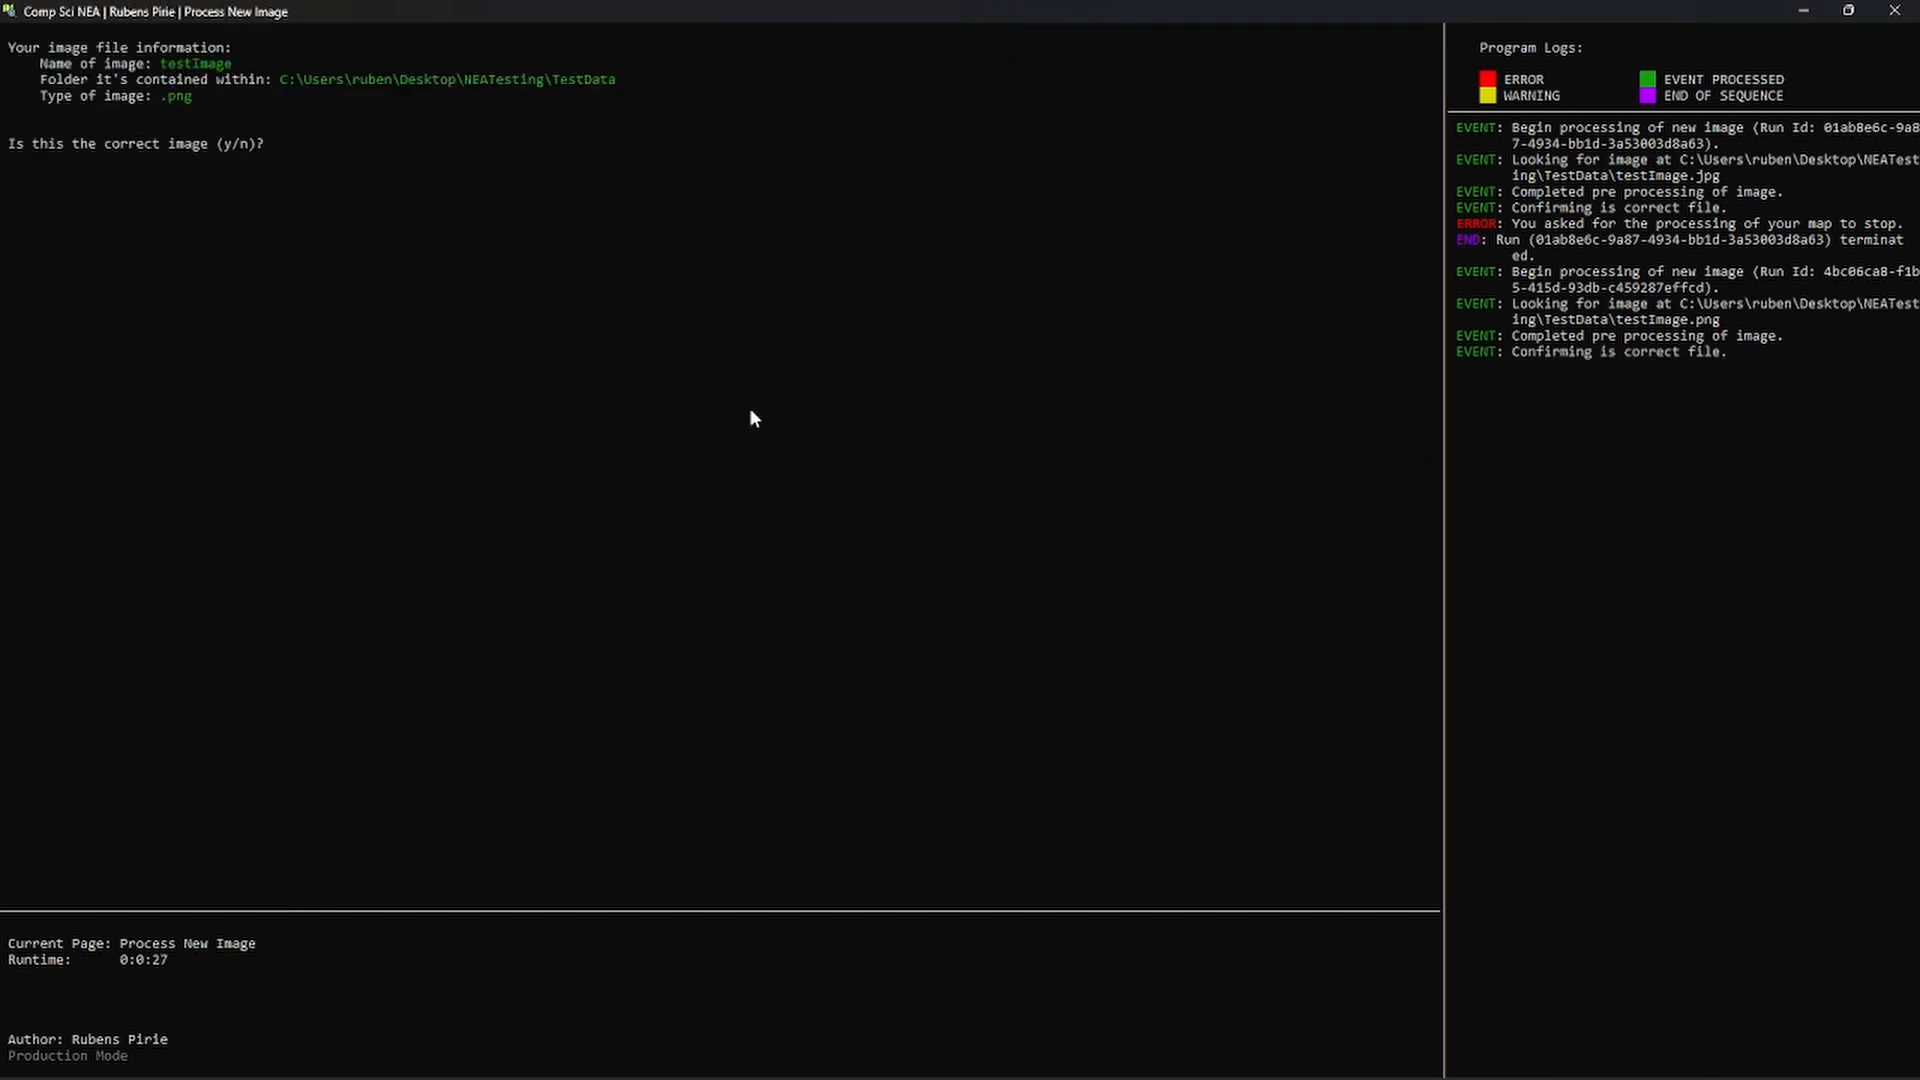
\includegraphics[width=12.5cm]{images/design/terminal.png}}}
    \end{figure}\\
    
    \BK

    \paragraph{Design of User Interface (Windows Forms)} \mbox{} \\
    For the forms interface I have chosen to keep the use of the opening of new windows to a minimum, as explained above I want this part of the program to be as simple as possible to avoid over stimulating the user and confusing them. 

    \begin{figure}[H]
        \centering
        \subfloat[\centering Windows Form For Confirming Image]{{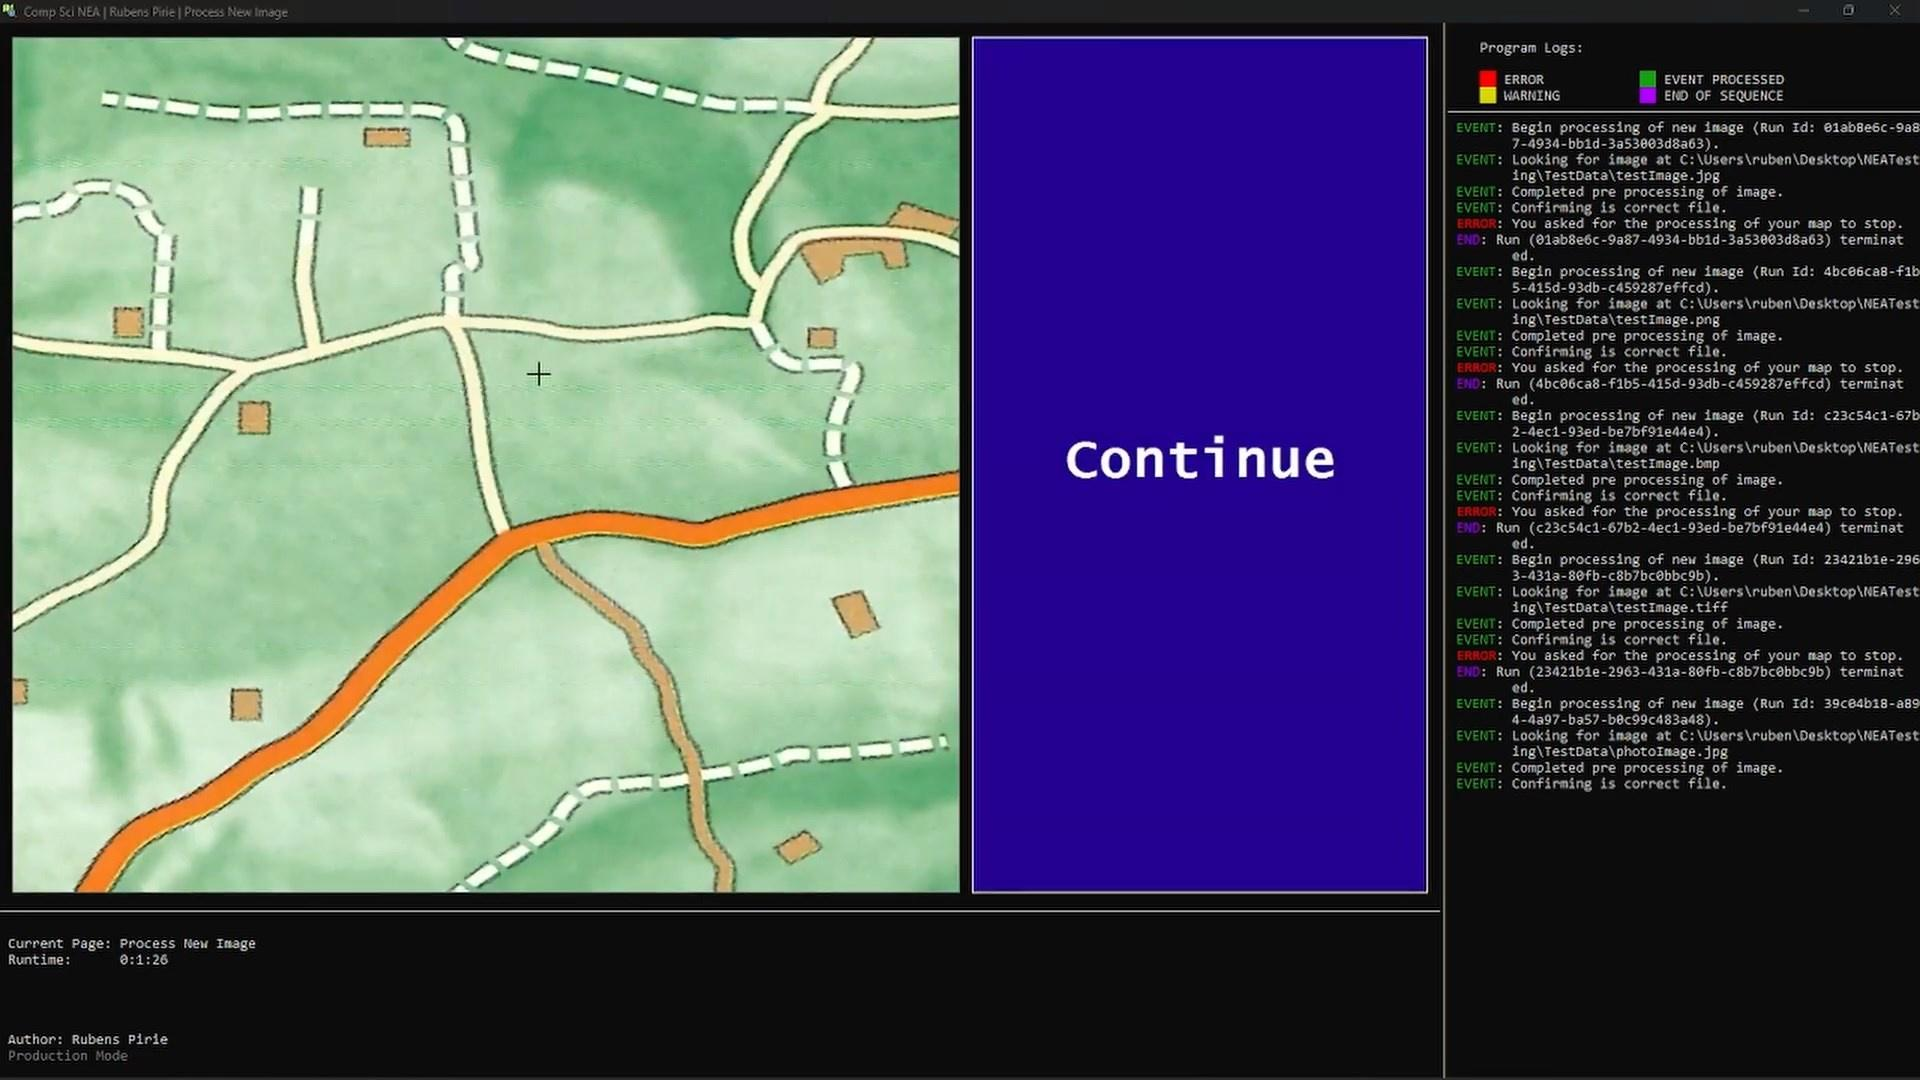
\includegraphics[width=12.5cm]{images/design/confirmWindow.jpeg}}}
    \end{figure}\\

    \begin{figure}[H]
        \centering
        \subfloat[\centering Windows Form For Pathfinding Image]{{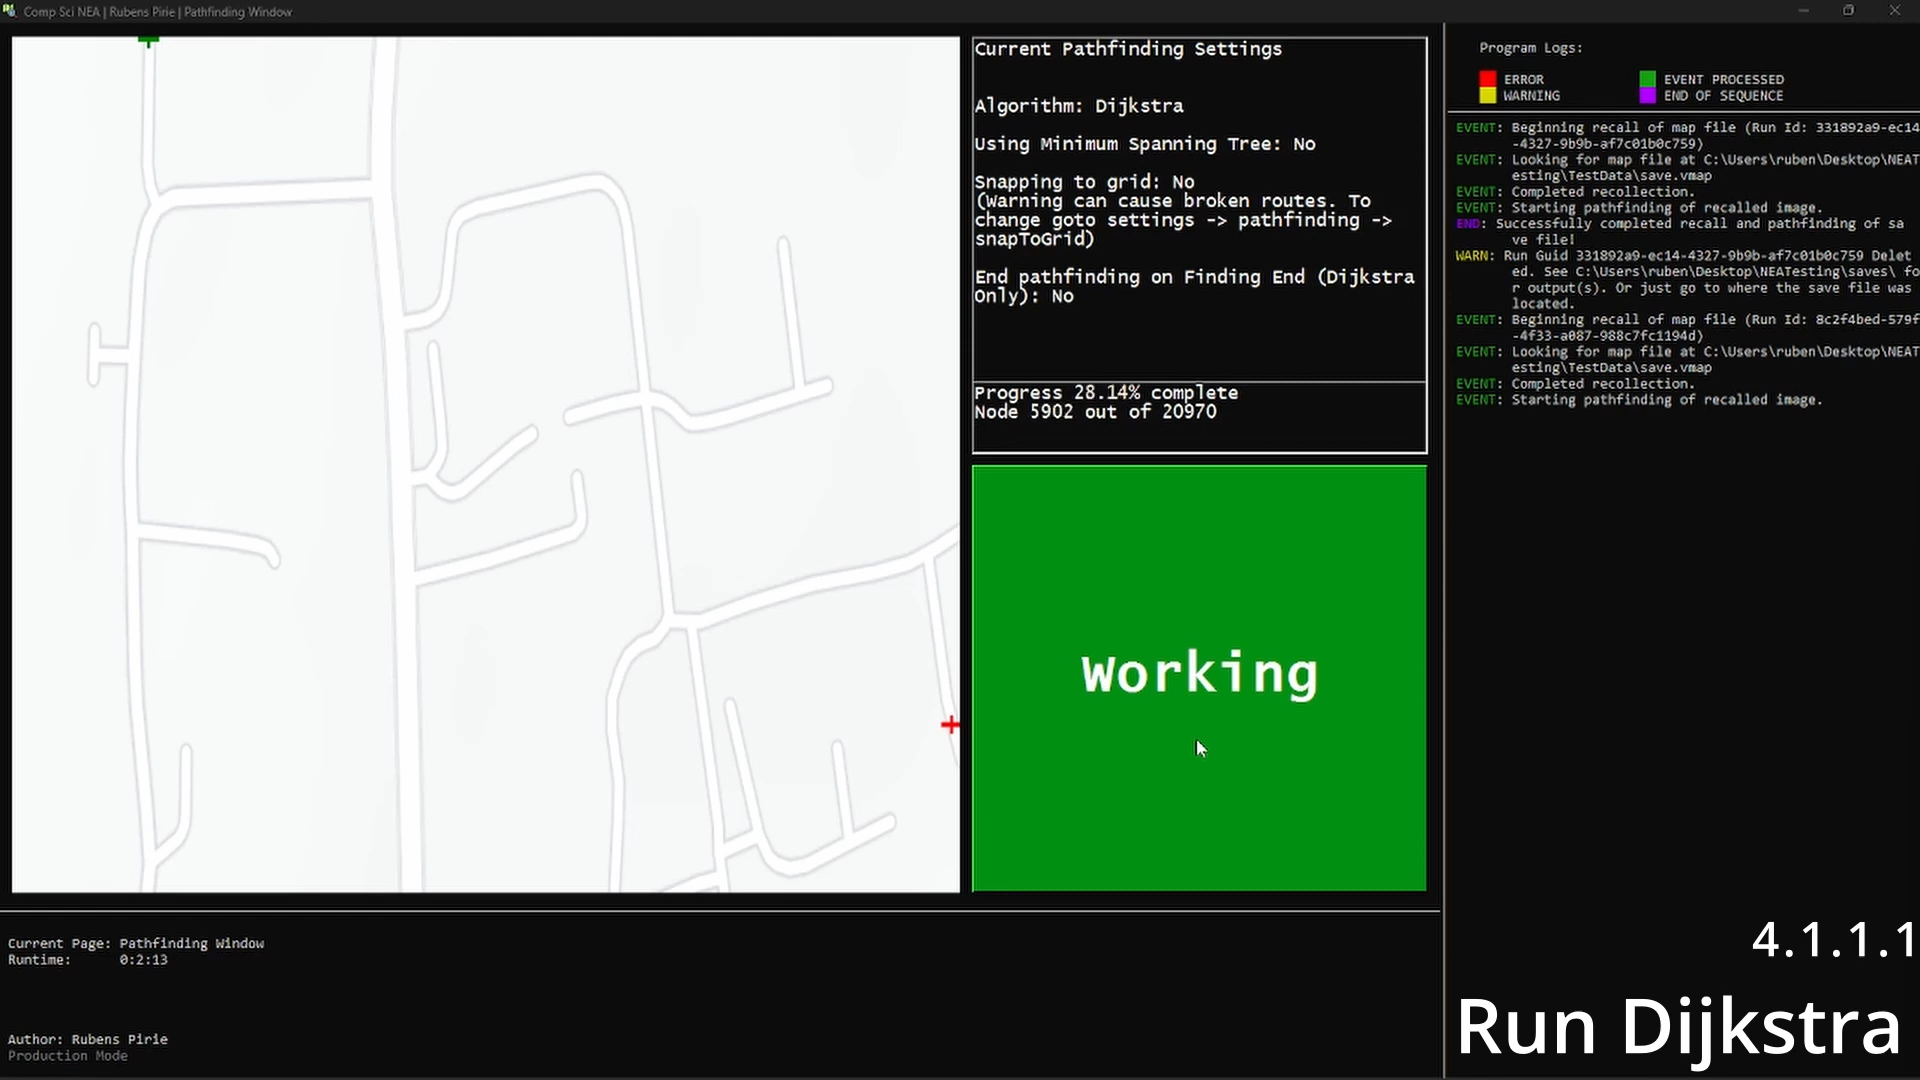
\includegraphics[width=12.5cm]{images/design/pathfindWindow.png}}}
    \end{figure}\\

    \\ \BK

    \subsubsection{Entire Class Diagram}
    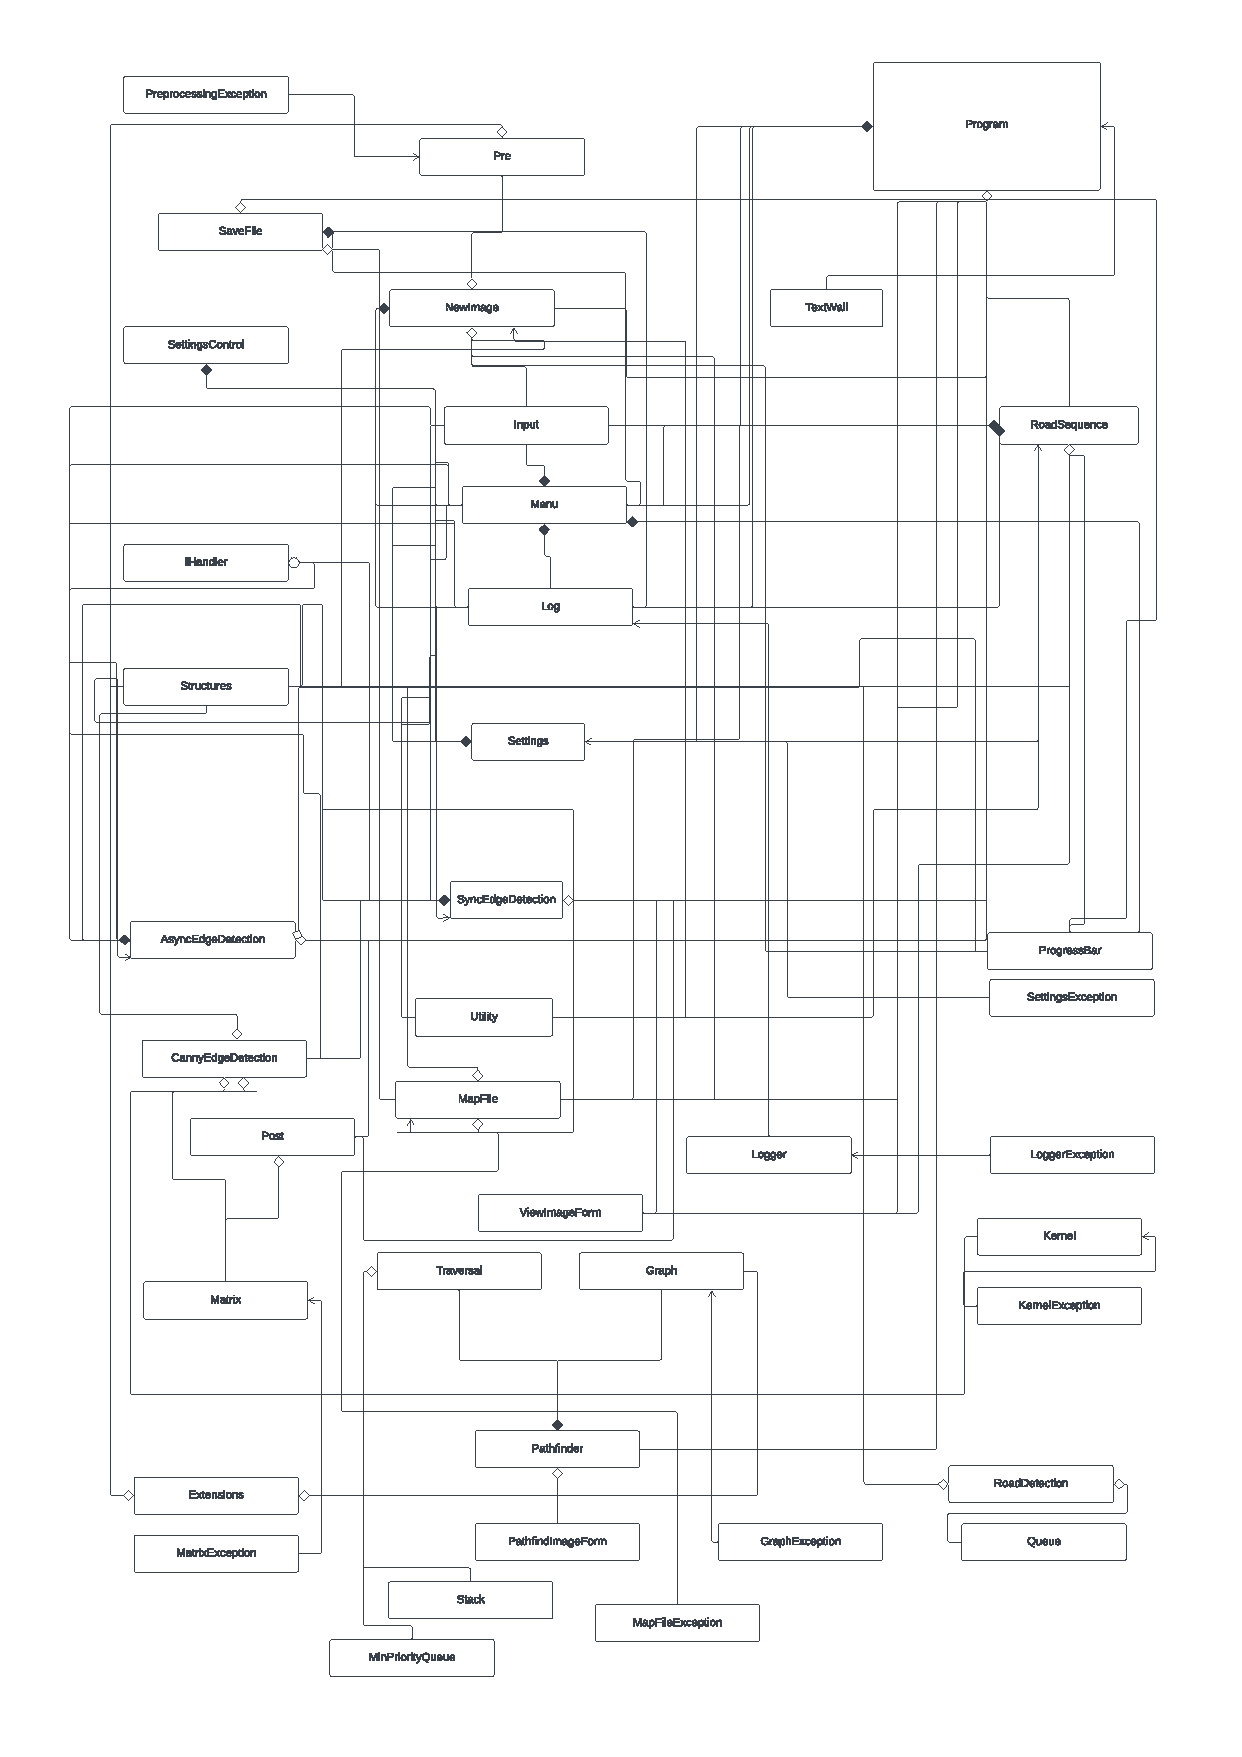
\includepdf{FullUML.pdf}
        
    \\ \bk

    \subsection{Binary File Structure}

    There will be an option during the process of the program for the user to save what they are doing with a binary file. Inside this file will be contained all of the information relating to the map. It will store, the name of the map, description, whether it needed to be inverted, date of creation, type of image, and 3 various versions of the image. \\ \bk

    The program will ask the user if they want to save the image, if they select yes to this then it will go on to ask them what the name of the map should be. A brief description to allow them to remember what it was for, and finally the type of map which can aid in future processing. These are all stored as strings apart from the type of map which is stored as a integer. \\ \bk

    The 3 images which are stored, these are the original image, the path found image, and the combined image which is the path overlays onto the original. These are all stored as bytes, this is to keep the size of the image to a minimum. This does raise the issue of there being no way to tell the size of the image. To overcome this there are two Int32's stored at the very beginning which are the dimensions of all the images meaning that it can be read without any guesswork. This has the effect of compressing all information relating to the images since each image's pixel is only 3 bytes. \\ 

    \subsection{Class Overviews}

    In this following part of the write up will go briefly over every class in the program first stating its function, which section it is in (backend library or front end application) and finally how it plays a part in the program.

    \paragraph{Async Edge Detection \textit{(Class)}} \mbox{} \\

    \begin{figure}[H]
        \centering
        \subfloat[\centering Async Edge Detection Class Diagram]{{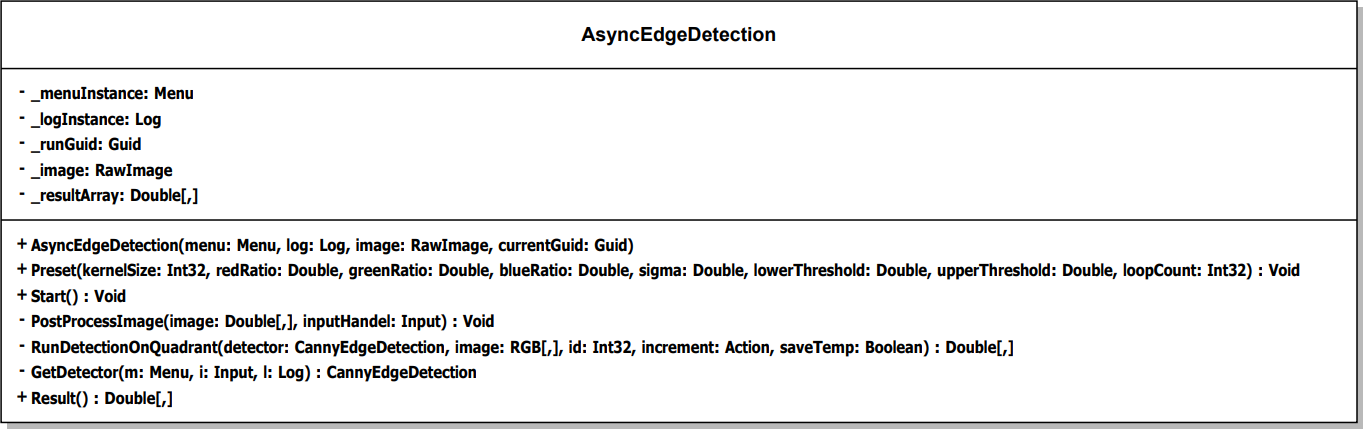
\includegraphics[width=16cm]{images/UML/AsyncEdgeDetection.png}}}
    \end{figure}\\

    This class is located in the front end section of my application, its main function is to coordinate the method calls of the Canny Edge Detection class. Due to the separated nature of my program I did not want there to be any user inputs in the accrual processing section. In order to do this I needed to have a separate hander on the local application side which would ask the user for their inputs and handel all of the validation of them. \\ \bk

    This class also implements the IHandler interface, this is to allow the main front end application to switch between the Async version and the Synchronous version of the edge detection without having a mess of IF statements. Part of the IHandler interface means that this class must contain the methods, Start() and Result(). What these methods do is what they say in the name. The start methods begins the process of getting user inputs and then starting the edge detection. The Result method will, as the name suggests return the result of the edge detection. \\ \bk

    The PostProcessImage method in the class is responsible for the custom embossing which runs through the result of the Canny edge detection and fills in any gaps that may have appeared. It also applies an embossing kernel on the image to embolden the lines. It will also prompt the user to enter the amount of times they want to run the embossing process. \\ \bk
    
    The GetDetectorMethod is used to get the variables for the Canny edge detector. This section handles all of the validation and checking that the values supplied are valid. The result of this method is that a new Canny Edge Detector object is created with the user inputted variables, this is then passed down the chain to be used in processing each quadrant. \\ \bk

    The main differentiator between this asynchronously method and the synchronous method is that this one will split the input image into 4 distinct quadrants, this will allow the program to run each at the same time using threading. Through my prototyping stage I found that using this method of threading greatly improves the speed even on lower specification computers. \\ \bk
    
    Finally the Preset method is used in the front end application in the eventuality of the user selecting preset values. An example of this is that when it gets to the selection of the edge detection method they select the "Photograph" method, the async method will be used due to its speed however instead of prompting the user it will run the various stages with predefined values. \\

    \bk
    \pagebreak
    \paragraph{Canny Edge Detection \textit{(Class)}} \mbox{} \\

    \begin{figure}[H]
        \centering
        \subfloat[\centering Canny Edge Detection Class Diagram]{{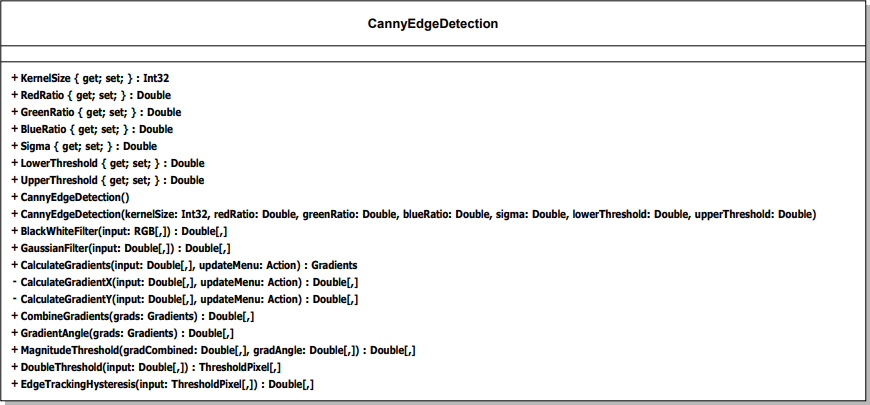
\includegraphics[width=16cm]{images/UML/CannyEdgeDetection.png}}}
    \end{figure}\\

    This class is located in the backend library portion of my project, its main function is to house the methods which contain the maths to perform the Canny edge detection. Since this method is in the backend library of my project there is no user input here however in many of the methods an action is passed in, this is used to update the progress bar on the front end without having the two intrinsically integrated. \\ \bk

    The first set of methods shown in the class diagram are in essence properties on the class which are used in the various calculations. The reason that I will go with getter and setter variables is that if at some point in the future I wish to restrict access to the properties on the class or perhaps mutate the way in which they are stored this could be easily done without the need to change many different things. \\ \bk

    The first method and subsequently the first stage in Canny edge detection is the black and white filter. The default behaviour is that it uses the industry standard for getting a single value from a RGB pixel which is as follows $$ Y' = 0.299R' + 0.587G' + 0.114B' $$.  It will perform the same calculation for every pixel in the supplied image causing it to be converted to black and white. This is used since if the detection was run on each colour chanel seperatly this would not give one unified result and could be very inaccurate.\\ 

    \\ \bk

    The next method in this class is the Gaussian Filter this will pass over the image and apply a Gaussian Filter kernel to each pixel. This is mainly used in order to make sure that any noise in the image is suppressed to avoid false edges. The maths for the kernel implementation and matrix convolutions are covered in their respective classes as well as the gaussian equation. A rough approximation for the gaussian kernel is as follows:\\

    \begin{gather*}
        \frac{1}{159}\begin{pmatrix}
            2 & 4 & 5 & 4 & 2 \\
            4 & 9 & 12 & 9 & 4 \\
            5 & 12 & 15 & 12 & 5 \\
            4 & 9 & 12 & 9 & 4 \\
            2 & 4 & 5 & 4 & 2
        \end{pmatrix}
    \end{gather*} \\

    It is stated that the larger the kernel is the less effect noise will have on the result however it will impact the performance of the detector, for this reason the Canny Edge Detection class defaults to a kernel size of 5x5. \\ \bk

    The next stage of Canny edge detection involve calculating gradients and gradient angles and for this reason I will be combining the CalculateGradients, CalculateGradientX and CalculateGradientY into one. Again another way in which I will optimise the Canny edge detection is by using threading. In order to calculate the gradient direction I will need to use Atan2, this requires an X and Y component which are independent of each other, a perfect use of threading. When a image gets to this point it will be processed at the same time by each method. The process completed by each method is vastly the same they will just be applying different image kernels, both are the sobel edge kernels keeping with the scheme of Canny edge detection. \\ \bk   

    \begin{center}
        
        $
        M_x = \begin{pmatrix}
            +1 & +2 & +1 \\
            0 & 0 & 0 \\
            -1 & -2 & -1
        \end{pmatrix}
    $ 
    and $ M_y = \begin{pmatrix}
            +1 & 0 & -1 \\
            +2 & 0 & -2 \\
            +1 & 0 & -1 
        \end{pmatrix}
    $
    \end{center} \\
 
    \bk

    Once the gradient magnitudes in each dimension have been calculated the result of these can be fed into the CombineGradients method. This method will finally extract the usefully data which has been created from applying the two sobel gradient kernels. The first of these is working out the combined gradient magnitudes which is simply calculated with the equation: \\
    
    \begin{gather*}
        G = \sqrt{G_x^2 + G_y^2}
    \end{gather*} \\
    
    We then also want to calculate the direction in which the gradient is travelling to work out if it is extreme enough to quantify an edge. This is achieved though the use of Atan2 as follows:\\
    
    \begin{gather*}
        \Theta = \text{Atan2}(G_x, G_y)
    \end{gather*} \\ 

    \bk

    The next stage in Canny edge detection is gradient magnitude threshold's, this is a method of removing lines which would not be "thick enough" to be a propped edge. This is accomplished by the use of the MagnitudeThreshold method and the bullet point description: \\ 
    
    At every pixel N in a given image, it will be suppressed (removed) if,
    \begin{itemize}
        \item the rounded gradient angle is 0° (i.e. the edge is in the north-south direction) the point will be considered to be on the edge if its gradient magnitude is greater than the magnitudes at pixels in the east and west directions.
        \item the rounded gradient angle is 90° (i.e. the edge is in the east-west direction) the point will be considered to be on the edge if its gradient magnitude is greater than the magnitudes at pixels in the north and south directions.
        \item the rounded gradient angle is 135° (i.e. the edge is in the northeast-southwest direction) the point will be considered to be on the edge if its gradient magnitude is greater than the magnitudes at pixels in the north-west and south-east directions.
        \item the rounded gradient angle is 45° (i.e. the edge is in the northwest-southeast direction) the point will be considered to be on the edge if its gradient magnitude is greater than the magnitudes at pixels in the north-east and south-west directions.

    \end{itemize}
    
    \\ \bk

    The penultimate method call is to Double Threshold suppression. After the magnitude threshold, remaining edge pixels provide a more accurate representation of real edges in an image. However, some edge pixels remain that are caused by noise and color variation which didn't get removed by the gaussian filter stage. To account for these spurious responses, it is essential to filter out edge pixels with a weak gradient value and preserve edge pixels with a high gradient value. \\

    The way in which this is implemented is that a user threshold from the beginning is used and if the pixel is greater than the threshold then it is included, if it is below the max threshold but greater than the min then it is set to a strong pixel and retains its value. In any other case it is removed and its value is set to 0. \\ \bk

    Finally edge tracking by hysteresis is used, to track the edge connection, blob analysis is applied by looking at a weak edge pixel and its 8-connected neighbourhood pixels. As long as there is one strong edge pixel that is involved in the blob, that weak edge point can be identified as one that should be preserved. These weak edge pixels become strong edges that can then cause their neighbouring weak edge pixels to be preserved otherwise they are not preserved and are removed. After each of these sages Canny edge detection is complete. \\ \bk    
    \bk

    \pagebreak
    \paragraph{Canny Result \textit{(Structure)}} \mbox{} \\

    \begin{figure}[H]
        \centering
        \subfloat[\centering Canny Result Class Diagram]{{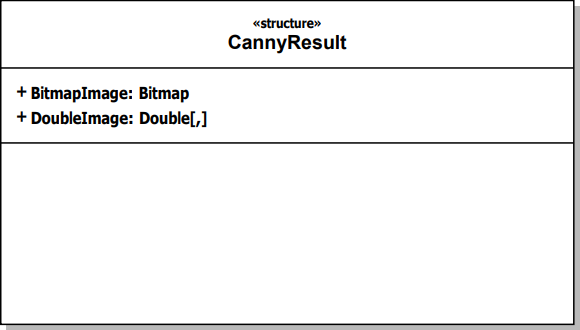
\includegraphics[width=10cm]{images/UML/CannyResult.png}}}
    \end{figure}\\

    This is contained within the static class of structures in the backend library. There is no methods or functions contained within this class since it is in fact a structure. Its main function is to contain any relevant data from Canny Edge Detection.

    \bk
    \pagebreak
    \paragraph{Coord \textit{(Structure)}} \mbox{} \\

    \begin{figure}[H]
        \centering
        \subfloat[\centering Coord Class Diagram]{{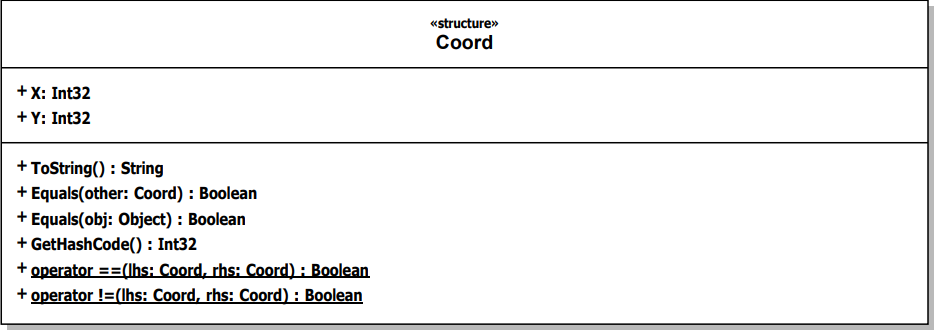
\includegraphics[width=13cm]{images/UML/Coord.png}}}
    \end{figure}\\

    Similar to above this is contained within the static class of structures. It is used to represent a coordinate, and unlike the Canny result structure, it does contain methods. The main of which are the operator overloads. This allows me to directly compare two different coordinates instead of constantly comparing each dimensions. The other hash codes and alike are used when a dictionary is required in order for them to be converted into a hash code. Finally the ToString method is mainly used during testing however it can also be used to inform the user of a coordinate that they are interacting with.

    \bk
    \pagebreak
    \paragraph{Extensions \textit{(Class)}} \mbox{} \\

    \begin{figure}[H]
        \centering
        \subfloat[\centering Extensions Class Diagram]{{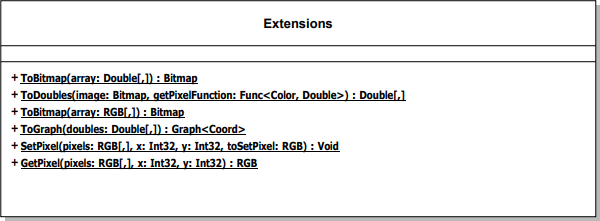
\includegraphics[width=13cm]{images/UML/Extensions.png}}}
    \end{figure}\\

    This class is responsible for altering the default behaviors of certain inbuilt classes in C# as well as extending functionality to make it easier to maintain my code. The way in which this is achieved is through the use of the this keyword. It will allow me for example to be to .ToBitmap on a 2D array speeding up the process instead of calling separate methods.\\ \bk

    The first of the extensions that will be implemented is the ToBitmap extension. As stated above it allows me to call ToBitmap on any given 2D double array, it then converts it to a bitmap and returns said bitmap. It does this through taking each pixel in turn and then using the Utility method to bound them within the allowed range of a pixel. \\ \bk

    Another of the extensions contained within this class is the ToDoubles extension which is essentially the inverse of the ToBitmap extension. This acts upon a Bitmap to convert it to a 2D double array. This extension however requires a method to be passed in which is then used to work out how to get the values of the pixel to a single 0 -> 255 value. The function which is passed in must take a Color object and return a single double value. \\ \bk

    The third extension contained is essentially a clone of the first one however this acts upon the EGB structure. This is important due to the fact that the RGB structure contains more than 1 value which means that using it I can reconstruct the original image using the R, G and B channels in the structure. Apart from this difference the two extensions are the same. \\ \bk

    The ToGraph extension contained within this class is very important as it is how after the Canny edge detection I will convert the result to a graph which can then have a traversal algorithm used upon it. This extension acts upon a 2D double array. In order to gain the pixels around a given pixel in a double array the GetKernel function is used, this is explained in the Kernel class. Once the kernel of the pixel is created we can work out the relative coordinates through the use of modulus arithmetic.

    \begin{gather*}
        \text{Where } X = x + (i \% 3) -1 \text{ and } Y = y + (i / 3) - 1 \\
    \end{gather*} \\ 

    Once this has been calculated more maths is done however this is contained within the graph class so see there for more information. \\ \bk

    The next two structures go hand in hand so I will talk about both of them together, due to the image processing and the way in which I am accessing the arrays which contain the data I feel that it would be easier if I could alter my RGB[,] and directly access it with the .setPixel and .getPixel methods since this is how it is used in the bitmap class. Therefore it would make it easier to use the two interchangeably instead of accessing it using direct accessing then changing the value. The way in which they both work is that in the function call an x and y coordinate is passed as well as a colour if it is the set pixel version. Then it changes or returns the value.\\    

    \bk
    \pagebreak
    \paragraph{Gradients \textit{(Structure)}} \mbox{} \\

    \begin{figure}[H]
        \centering
        \subfloat[\centering Gradients Class Diagram]{{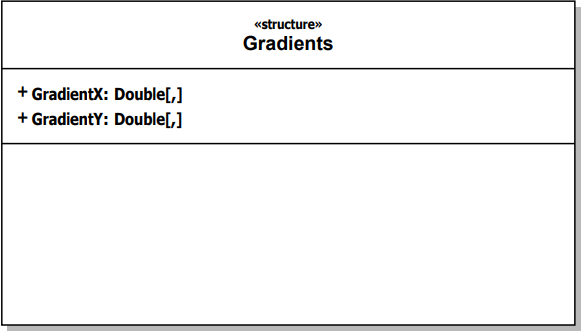
\includegraphics[width=10cm]{images/UML/Gradients.png}}}
    \end{figure}\\

    This is a structure located in the back end library of my project, its main function in the program is store the result of the gradient calculations. As with many of my structures in this code, there is no methods contained within. 

    \bk

    \pagebreak
    \paragraph{Graph \textit{(Class)}} \mbox{} \\

    \begin{figure}[H]
        \centering
        \subfloat[\centering Graph Class Diagram]{{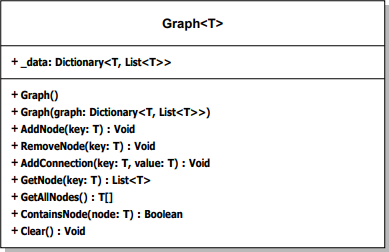
\includegraphics[width=10cm]{images/UML/Graph.png}}}
    \end{figure}\\

    The graph class is located in the backend portion of the project. Its responsible for holding all node data corresponding to a graph. The general implementation of this graph class is rather basic however it is responsible for allowing the majority of the program to work. All of the methods inside the class are generics. This means that a graph of any data type can be created. This especially usefully in my case because it allows me to have the nodes as Coordinate structures meaning that I can easily get its corresponding point on a map image. \\ \bk

    The methods included in this class are as follows:
    \begin{itemize}
        \item AddNode - As the name suggests this is responsible for adding a node to the graph. You cannot add neighbors in the same function, you pass in the node name.
        \item RemoveNode - This is the partner method to the one above which removes a node from the graph deleting all of its neighbors connections.
        \item AddConnection - This ties an existing node to the on the graph to an existing node. This allows us to tell where a node can go to from its current one.
        \item GetNode - This allows the program to fetch a single node from the graph. It will only return connections on the node.
        \item GetAllNodes - Returns all nodes in the graph including those, if they exist, which have no neighbors.
        \item ContainsNode - Allows the program to easily check if a node exists, this is an optimisation to allow the program to run faster and at a higher level of abstraction.
        \item Clear - Clears the node
    \end{itemize}

    \bk
    \pagebreak
    \paragraph{Graph Exception \textit{(Exception)}} \mbox{} \\

    \begin{figure}[H]
        \centering
        \subfloat[\centering Graph Exception Class Diagram]{{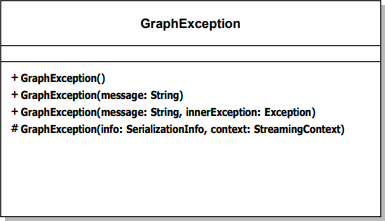
\includegraphics[width=10cm]{images/UML/GraphException.png}}}
    \end{figure}\\

    Located in the backend of the project this is a specific exception used to differentiate errors in the front end. This inherits the methods of the base exception class. This is the same as all other custom exception classes. They exist to allow me in the front end to show special error messages.

    \bk
    \pagebreak
    \paragraph{IHandler \textit{(Interface)}} \mbox{} \\

    \begin{figure}[H]
        \centering
        \subfloat[\centering IHandler UML Diagram]{{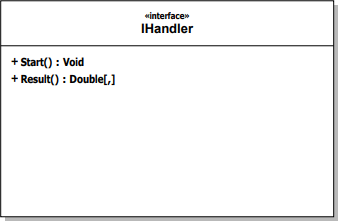
\includegraphics[width=10cm]{images/UML/IHandler.png  }}}
    \end{figure}\\

    This is located in the backend portion of the program. IT itself has no code due to the fact that it is an interface and is soule use is to cut down on code during the selection between async or synchronous edge detection. It requires all child classes to implement the functions, Start and Result. These will be used to as the names suggest start the process and get the result of the process. \\ \bk

    The advantage to using an interface here means that the object can be cast to a simplified version meaning that two different classes can be assigned to the same variable removing the need for guard clauses. \\
    \bk

    \pagebreak
    \paragraph{Input \textit{(Class)}} \mbox{} \\

    \begin{figure}[H]
        \centering
        \subfloat[\centering Input Class Diagram]{{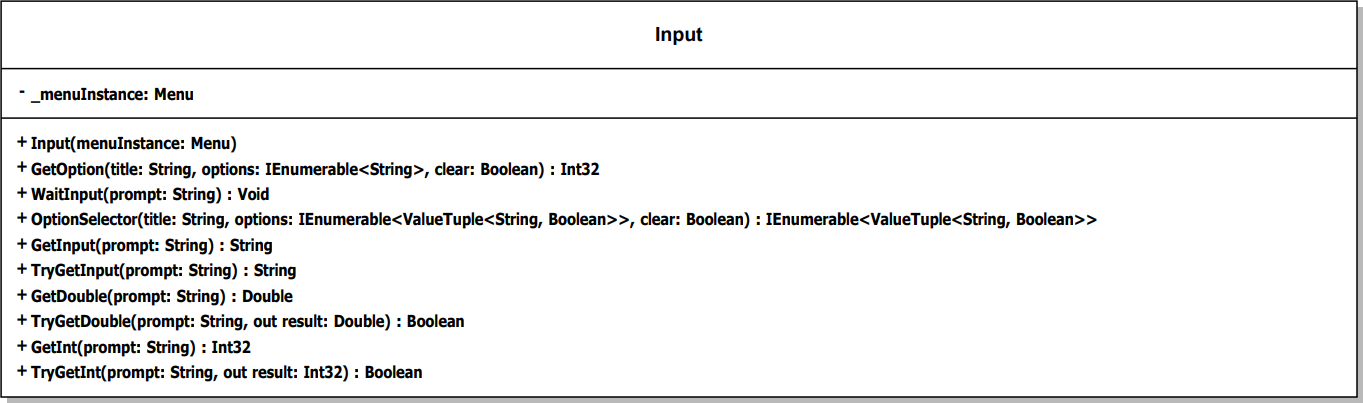
\includegraphics[width=15cm]{images/UML/Input.png}}}
    \end{figure}\\

    This is responsible for allowing the user to interact with the program and is an integral part. It is located in the front end of the project due to the fact that it is dealing with the user input. There are several functions in this class which act in different ways. \\ \bk

    One of the integral functions of the program is to be able to get the user to select an option from a list of options. The function works by taking an IEnumerable of strings which are the options. Once the user has selected an option th function returns the 0-indexed reference to the option that was selected. \\ \bk

    The WaitInput method is soul's used for waiting for the ser to press any key to move on. This can be used when waiting for the user to read something without there having to be an arbitrary time delay. \\ \bk

    The OptionSelector method is used in the setting section of the program. This method will take an IEnumerable of tuples which are used for settings. It allows the user to press the enter or space-bar key which changes the boolean value of a string. This can be used to change the "SaveToZip" file. Once the user has completed all of their setting changes and choses to exit the function will return the same IEnumerable with the changed boolean values. \\ \bk

    The following functions GetInput, TryGetInput, TryGetInt, TryGetDouble, GetInt and GetDouble are all used as the name suggests to get user input. The Try version of the methods instead return a boolean if the getting of the input was successful. These echo the double.TryGet in c# however instead they are tied into the custom menu system of the program. The non Try versions will throw an exception if they are unsuccessful in getting the input which will need to be handled further up the call stack.\\ 

    \bk

    \pagebreak
    \paragraph{Kernel \textit{(Class)}} \mbox{} \\

    \begin{figure}[H]
        \centering
        \subfloat[\centering Kernel Class Diagram]{{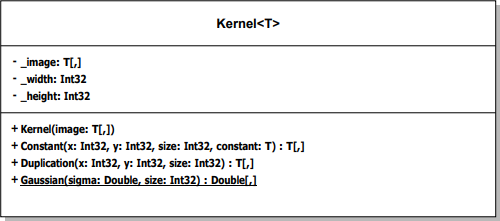
\includegraphics[width=10cm]{images/UML/Kernel.png}}}
    \end{figure}\\

    This is the class which is responsible for generating image kernels from a supplied image. This is also writer with generics meaning that the kernel will be able to be generated from and 2D array. This was especially usefully when it came down to using both doubles to represent black and white pixels and Color objects which represent an RGB pixel. \\ \bk

    This class implements two types of fetching the kernel, the first of which is Constant and the second of which is Duplication. The first method, duplication runs the exact same as the second method, it will take in the center of the kernel and the size. It will run a loop over the "area" of the desired kernel if the coordinate is inside the bound of the image then it will use that in the kernel however if it is not in the duplication version it will take the initial kernel and duplicate that. This is explained in more detail in the analysis section when I was investigation this field. The constants version will just use a constant value which in this  case is 128 which is a grey colour in black and white. \\ \bk

    The resulting kernel is then converted into a matrix and retuned in order to be convoluted with the processing kernel. The only exception to this is the gaussian kernel. This does not take in an image, instead it applies the 3D statistical gaussian distribution to a matrix producing a 3D Gaussian distribution matrix of a given size. This is then returned to be used in the Canny edge detection section.\\
    \bk

    \paragraph{Kernel Exception \textit{(Exception)}} \mbox{} \\

    \begin{figure}[H]
        \centering
        \subfloat[\centering Kernel Exception Class Diagram]{{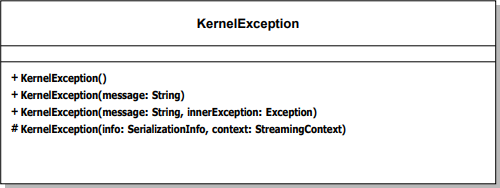
\includegraphics[width=12.5cm]{images/UML/KernelException.png}}}
    \end{figure}\\
    Located in the backend of the project this is a specific exception used to differentiate errors in the front end. This inherits the methods of the base exception class. This is the same as all other custom exception classes. They exist to allow me in the front end to show special error messages.

    \bk
    \pagebreak
    \paragraph{Log \textit{(Class)}} \mbox{} \\

    \begin{figure}[H]
        \centering
        \subfloat[\centering Log Class Diagram]{{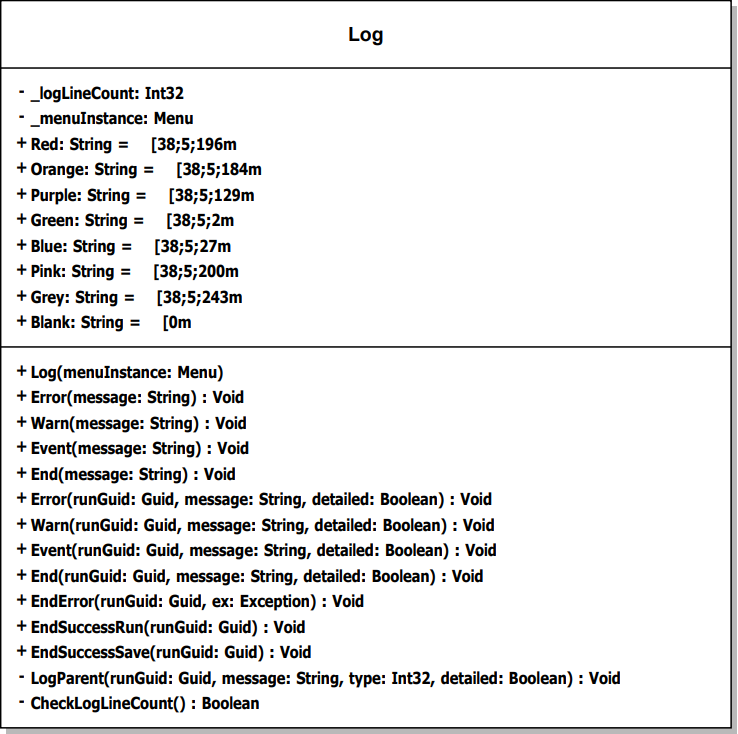
\includegraphics[width=12.5cm]{images/UML/Log.png}}}
    \end{figure}\\

    The Log class is located in the front end of the program due to the fact that it is interacting with the user, there is also a Logger class, this is responsible for the outputs and is located back end and is explained below. Most of the methods contained within this class do the same thing by printing a log message however there are two distinct versions. \\ \bk

    The first of are the methods which contain only a message as an argument, these logs are not displayed to the user and are instead sent directly to a save file to be logged. I chose to do this because it will allow me to hide some complexity to the user. \\ \bk

    The second version of the log is the one which if detailed logging is enabled will be shown to the user. There is a case in this method however in which the setting can be overridden. This means that for important messages like the beginning and end will be shown even if the user wants it or not. \\ \bk

    The end success and end error functions are used to end a run which as stated above overrides the logging and forces it to the side. It also saves the outputs and manages all of the file structures. \\ \bk

    There are several static properties of the class these are the ascii colour codes which are used to make the user interface more palatable to the user. The over very important property is the current line, this allows the program to tell how far down the log side it is and to see if it needs to be cleared. It is incremented every time a new line is logged. \\

    \bk
    \pagebreak
    \paragraph{Logger \textit{(Class)}} \mbox{} \\

    \begin{figure}[H]
        \centering
        \subfloat[\centering Logger Class Diagram]{{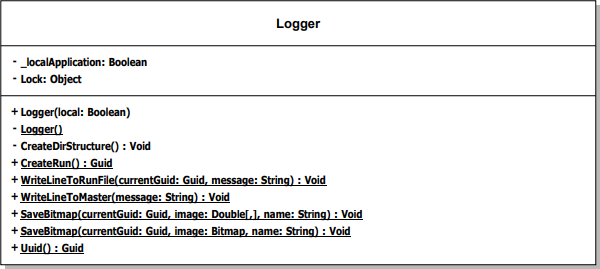
\includegraphics[width=14cm]{images/UML/Logger.png}}}
    \end{figure}\\

    This is the part of the code which is responsible for saving all of the users files which have been generated though the program. Since the methods contained within are rather generic in how they could function I will bullet point the general idea behind each one.

    \begin{itemize}
        \item CreateDirStructure - As the name suggests this creates the desired directly structure for the user depending on how the designer wishes it to be laid out. This checks if the directories exist and if they don't then it creates them. This is not responsible for creating any of the files used in the program like settings.conf or master.log
        \item CreateRun - The use for this is to create a run, this will create a directory, in this program, inside the runs folder. It also will create a run log file with a random guid. This guid is then returned to be used in the rest of the program and when logging.
        \item WriteLineToLogFile - Writes a line to a log file given a UUID / Guid. It will locate the file and append it to the end. 
        \item WriteLineToMaster - This will append a line to the master log file which is located in this case inside the logs directory.
        \item SaveBitmap - Both the functions here will save a bitmap into a folder given a GUID, if the double array is supplied then it converts to a bitmap then it is saved. If a bitmap is supplied the bitmap is saved.
        \item Uuid - Returns a new UUID also known as a GUID
    \end{itemize}

    \bk
    \pagebreak
    \paragraph{Logger Exception \textit{(Exception)}} \mbox{} \\

    \begin{figure}[H]
        \centering
        \subfloat[\centering Logger Exception Class Diagram]{{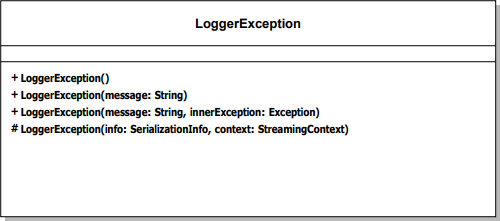
\includegraphics[width=10cm]{images/UML/LoggerException.png}}}
    \end{figure}\\
    Located in the backend of the project this is a specific exception used to differentiate errors in the front end. This inherits the methods of the base exception class. This is the same as all other custom exception classes. They exist to allow me in the front end to show special error messages.
    \bk
    \pagebreak
    \paragraph{Map File \textit{(Class)}} \mbox{} \\

    \begin{figure}[H]
        \centering
        \subfloat[\centering Map File Class Diagram]{{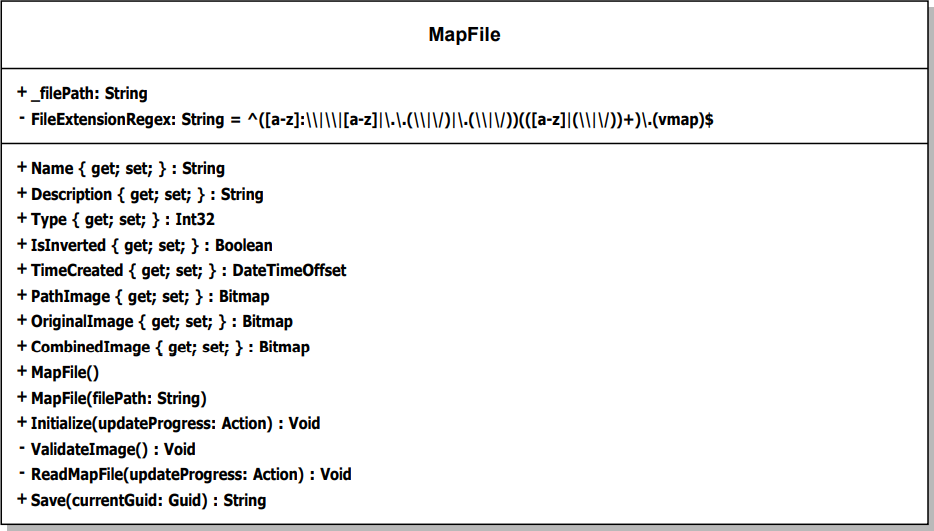
\includegraphics[width=15cm]{images/UML/MapFile.png}}}
    \end{figure}\\

    This is located in the backend library of the project. Its function is to store and create map save files.All of the methods contained within with the suffix { get; set;} are actual properties on the class which are used to store information about the save file. \\ \bk

    The file extension regex is part of the properties is used to validate whether a given file is actually a map file. This comes in usefully when recalling a map from a save file. This is when the method Initialize comes in useful, it takes in the file path, validates it and then according to a set of rules will read in the custom binary file, the actual reading of the map fle is done in the ReadMapFile method. However this is called from within the validate function since we only want this to run if the file is valid. \\ \bk

    If at any point it encounters an error it will throw an exception which tells the user what the issue is. The final function of this class is saving the map file. This is done once all processing has been done, it saves it using a binary file. It is important to me that the file was all in one place and not split up allowing it to be transferred easily. \\ 
    \bk

    \pagebreak
    \paragraph{Map File Exception \textit{(Exception)}} \mbox{} \\

    \begin{figure}[H]
        \centering
        \subfloat[\centering Map File Exception Class Diagram]{{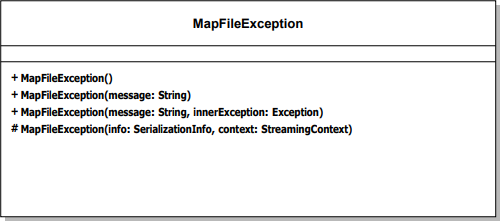
\includegraphics[width=12.5cm]{images/UML/MapFileException.png}}}
    \end{figure}\\
    Located in the backend of the project this is a specific exception used to differentiate errors in the front end. This inherits the methods of the base exception class. This is the same as all other custom exception classes. They exist to allow me in the front end to show special error messages.
    \bk
    \pagebreak
    \paragraph{Matrix \textit{(Class)}} \mbox{} \\

    \begin{figure}[H]
        \centering
        \subfloat[\centering Matrix Class Diagram]{{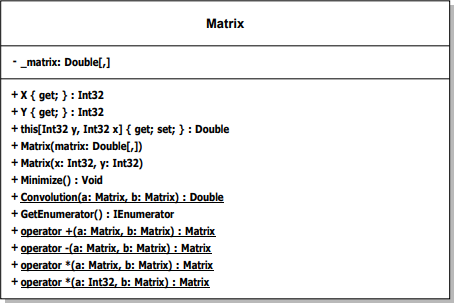
\includegraphics[width=12.5cm]{images/UML/Matrix.png}}}
    \end{figure}\\

    This is located in the backend portion of my program. Again as above the methods of the class which are responsible for storing data to do with the program are denoted with { get; set; }. The X and Y properties of the matrix class denote the dimensions of the matrix. \\ \bk
    
    There is a direct array access to the data in the matrix. This was so that when assigning the gaussian distribution to a new matrix I would have to have stored all of the values in a temporary 2D array just for it to be assigned to a matrix. Therefore I made the decision to allow my program to directly access the cells of the matrix through the [] notation. It is both Get and Set however it could be made internal to keep the library and the front end even more separated. \\ \bk

    There is a rather large amount of operator overloading in this section which perform the various numerical operations of the matrix. These are as follows: \\ \bk

    \textbf{Matrix Addition} \\ \bk
    {\displaystyle {\begin{aligned}\mathbf {A} +\mathbf {B} &={\begin{bmatrix}a_{11}&a_{12}&\cdots &a_{1n}\\a_{21}&a_{22}&\cdots &a_{2n}\\\vdots &\vdots &\ddots &\vdots \\a_{m1}&a_{m2}&\cdots &a_{mn}\\\end{bmatrix}}+{\begin{bmatrix}b_{11}&b_{12}&\cdots &b_{1n}\\b_{21}&b_{22}&\cdots &b_{2n}\\\vdots &\vdots &\ddots &\vdots \\b_{m1}&b_{m2}&\cdots &b_{mn}\\\end{bmatrix}}&={\begin{bmatrix}a_{11}+b_{11}&a_{12}+b_{12}&\cdots &a_{1n}+b_{1n}\\a_{21}+b_{21}&a_{22}+b_{22}&\cdots &a_{2n}+b_{2n}\\\vdots &\vdots &\ddots &\vdots \\a_{m1}+b_{m1}&a_{m2}+b_{m2}&\cdots &a_{mn}+b_{mn}\\\end{bmatrix}}\\\end{aligned}}\,\!}\BK\BK\bk

    \BK
    \textbf{Matrix Multiplication} \\ \bk
    Let 
    {\displaystyle \mathbf {A} ={\begin{pmatrix}a_{11}&a_{12}&\cdots &a_{1n}\\a_{21}&a_{22}&\cdots &a_{2n}\\\vdots &\vdots &\ddots &\vdots \\a_{m1}&a_{m2}&\cdots &a_{mn}\\\end{pmatrix}},\quad \mathbf {B} ={\begin{pmatrix}b_{11}&b_{12}&\cdots &b_{1p}\\b_{21}&b_{22}&\cdots &b_{2p}\\\vdots &\vdots &\ddots &\vdots \\b_{n1}&b_{n2}&\cdots &b_{np}\\\end{pmatrix}}}

    
    {\displaystyle \mathbf \therefore {C} ={\begin{pmatrix}a_{11}b_{11}+\cdots +a_{1n}b_{n1}&a_{11}b_{12}+\cdots +a_{1n}b_{n2}&\cdots &a_{11}b_{1p}+\cdots +a_{1n}b_{np}\\a_{21}b_{11}+\cdots +a_{2n}b_{n1}&a_{21}b_{12}+\cdots +a_{2n}b_{n2}&\cdots &a_{21}b_{1p}+\cdots +a_{2n}b_{np}\\\vdots &\vdots &\ddots &\vdots \\a_{m1}b_{11}+\cdots +a_{mn}b_{n1}&a_{m1}b_{12}+\cdots +a_{mn}b_{n2}&\cdots &a_{m1}b_{1p}+\cdots +a_{mn}b_{np}\\\end{pmatrix}}} \BK\BK\bk

    \textbf{Scalar Multiplication} \\ \bk
    \lambda \mathbf {A} =\lambda {\begin{pmatrix}A_{11}&A_{12}&\cdots &A_{1m}\\A_{21}&A_{22}&\cdots &A_{2m}\\\vdots &\vdots &\ddots &\vdots \\A_{n1}&A_{n2}&\cdots &A_{nm}\\\end{pmatrix}}={\begin{pmatrix}\lambda A_{11}&\lambda A_{12}&\cdots &\lambda A_{1m}\\\lambda A_{21}&\lambda A_{22}&\cdots &\lambda A_{2m}\\\vdots &\vdots &\ddots &\vdots \\\lambda A_{n1}&\lambda A_{n2}&\cdots &\lambda A_{nm}\\\end{pmatrix}} \BK\BK\bk

    \textbf{Matrix Convolution} \\ \bk
    This is very important for my program since this is the section which allows all of the image processing to function. The general form of matrix convolution is as follows:\\\bk

    {\displaystyle {\begin{bmatrix}x_{11}&x_{12}&\cdots &x_{1n}\\x_{21}&x_{22}&\cdots &x_{2n}\\\vdots &\vdots &\ddots &\vdots \\x_{m1}&x_{m2}&\cdots &x_{mn}\\\end{bmatrix}}*{\begin{bmatrix}y_{11}&y_{12}&\cdots &y_{1n}\\y_{21}&y_{22}&\cdots &y_{2n}\\\vdots &\vdots &\ddots &\vdots \\y_{m1}&y_{m2}&\cdots &y_{mn}\\\end{bmatrix}}=\sum _{i=0}^{m-1}\sum _{j=0}^{n-1}x_{(m-i)(n-j)}y_{(1+i)(1+j)}}\BK\BK\bk

    \textbf{Matrix Minimisation} \\ \bk
    This is more of a custom made algorithm. It runs over every entry in the matrix summing their values together. This is then used to divide every element in the matrix by this sum. This means that all of the elements will sum to zero if added which can help with matrix convolution. \\
    \bk

    \pagebreak
\paragraph{Matrix Exception \textit{(Exception)}} \mbox{} \\

    \begin{figure}[H]
        \centering
        \subfloat[\centering Matrix Exception Class Diagram]{{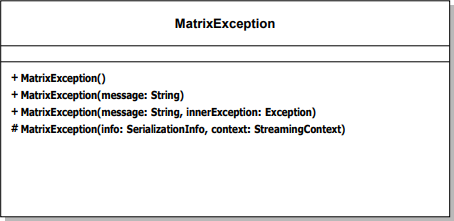
\includegraphics[width=12.5cm]{images/UML/MatrixException.png}}}
    \end{figure}\\
    Located in the backend of the project this is a specific exception used to differentiate errors in the front end. This inherits the methods of the base exception class. This is the same as all other custom exception classes. They exist to allow me in the front end to show special error messages.
    \bk


    \pagebreak
\paragraph{Max Priority Queue \textit{(Class)}} \mbox{} \\

    \begin{figure}[H]
        \centering
        \subfloat[\centering Max Priority Queue Class Diagram]{{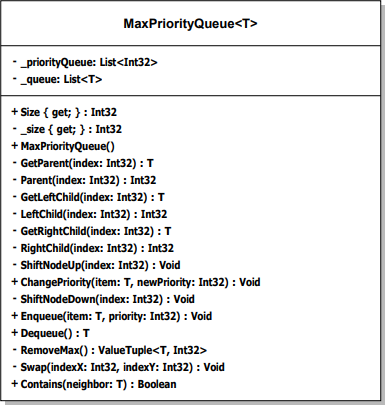
\includegraphics[width=9cm]{images/UML/MaxPriorityQueue.png}}}
    \end{figure}\\
    
    Again located in the back end library of the project, this is a data type used in the processing and pathfinding of the map. This is identical to the Min priority queue explained below apart from the ordering of the elements in the queue. Both use a binary heap. Please refer to the min priority queue for an explication of the methods involved.


    \bk

    \pagebreak
\paragraph{Menu \textit{(Class)}} \mbox{} \\

    \begin{figure}[H]
        \centering
        \subfloat[\centering Menu Class Diagram]{{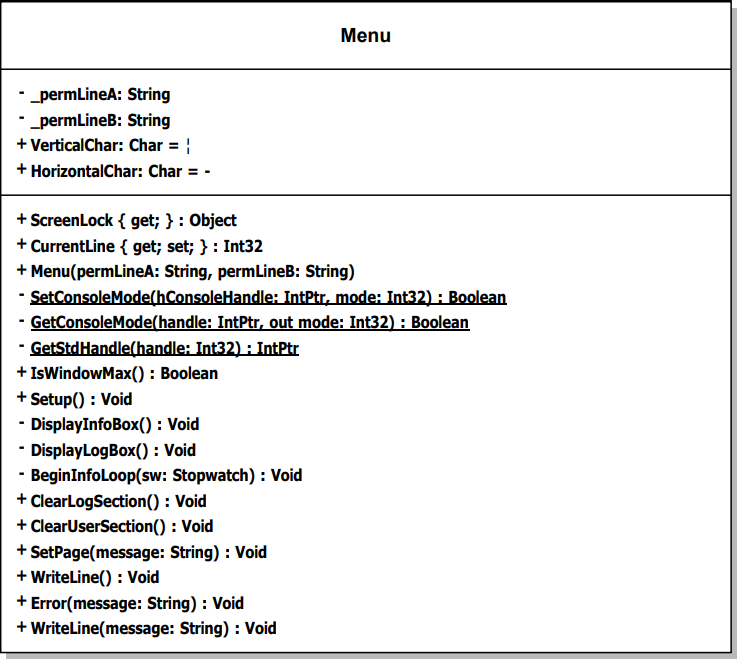
\includegraphics[width=13cm]{images/UML/Menu.png}}}
    \end{figure}\\

    This is located in the front end portion of my project and is responsible for most if not all of the CLI. There are multiple properties on this class which are used to set permanent display info. The first of these are \_permLineA and \_permLineB. These are used to show titles on screen to the user. In this case they are being used to display the title of the program and my name. The VerticalChar and HorizontalChar are used when drawing outlines onto the console screen. In this case they are a solid | and -. \\ \bk

    Also contained within the properties is a Lock object, this is used and is vital in order to prevent the screen from getting flooded by different colours and wrong sections of text. Due to the nature of threading, different threads can be used at any one time. This object is accessible anywhere in the front end section of the project. The CurrentLine integer is also vital since it lets the program keep track of where the next line needs to be drawn on the screen in the event a message needs to be sent to the user.\\ \bk

    The IsWindowMax function is used to make sure that the program will not start until the screen is as large as it can be, I decided to do this in order to make the most of the screen and keep the UI as simple for th user as possible, it employs use of the inbuilt windows API to allow me to check the dimensions of the screen. \\ \bk

    Since part of my program heavily interacts with the user I though that it was important to make sure that the UI was as inviting as possible. In order to do this I wanted to bring some colour into it, this is not possible in the base console since there is only 4 bit colour giving 16 possibilities. There is a way to enable 8 bit colour in the console through the use of console modes. This is the function of SetConsoleMode, GetConsoleMode, GetStdHandel and Setup. Each of those changes unique windows setting to allow for the use of ansi escape codes which are stored in the Log class. \\ \bk

    There are a verity of plain setup functions in this class who just create the boundaries for the various information boxes. These include, ClearLogSection, ClearUserSection, DisplayInfoBox and DisplayInfoBox, as the names suggest each of these creates a separate area in the console which can be seen above as an final image. The clear functions are called whoever the program requests it or there is too much information being displayed on the screen at any given time. An example of when there may be too much information is after there has been a long run performed where the user has selected advanced logging, the side bar will clear when the messages get to the bottom and return to the top. \\ \bk

    The BeginInfoLoop function is responsible for the timer which runs in the "Info" box telling the user if the program is running and if it has encountered a hang where, in which, the timer would stop as an indication that the program has encountered an error. There is also the SetPage function which sets the title and information page title allowing the user to know where they are at every stage.\\ \bk

    Finally there are the actual functions which display information to the user, WriteLine is a function which similar to the inbuilt Console.WriteLine displays a message to the user. If the line goes over the user section the program automatically crops it onto another line. There is also a version of this method which takes no arguments which is used for adding a break in between lines. This is needed due to a limitation with '\n'.

    \bk
    
    \pagebreak
\paragraph{Min Priority Queue \textit{(Class)}} \mbox{} \\

    \begin{figure}[H]
        \centering
        \subfloat[\centering Min Priority Queue Class Diagram]{{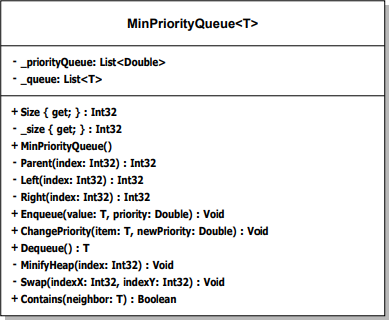
\includegraphics[width=10cm]{images/UML/MinPriorityQueue.png}}}
    \end{figure}\\

    This is perhaps one of the most important classes in the back end library. It is responsible for the speed and performance of the graph traversal. It is based upon a binary heap, this was chosen as it has a good ballance between complexity and performance. I will go over each method in turn describe the mathematics behind how it is stored. \\ \bk

    \textbf{Parent} \\ \bk
    The parent of a node can be found by doing $$ \frac{i - 1}{2}$$ this can be useful when shifting nodes around. \\ \bk

    \textbf{Left} \\ \bk
    The left node can be found by doing $$ (i * 2) + 1$$ this can be useful when finding where a node belongs in the queue.\\ \bk

    \textbf{Right} \\ \bk
    The right node can be found by doing $$ (2 * i) + 2$$ the same reasons as above. \\ \bk

    \textbf{ChangePriority} \\ \bk
    The change priority function in this class is very important since it can allow the program to change the priority on the fly when performing A* search. the way which A* functions is via using a hubristic function, this function changes with the position of the nodes on the graph therefore it may be that the value of the pixel in the queue needs to be changed this is where this method is used.  \\ \bk

    \textbf{Enqueue} \\ \bk
    Adds a node to the queue with a priority and a name. This is added into the correct position depending on its propriety.\\ \bk

    \textbf{Dequeue} \\ \bk
    This removes the front node from the queue, in this case this node will be the one with least value as its priority. This is how the A* search gets the next lowest node quickly.\\ \bk

    \textbf{MinifyHeap} \\ \bk
    This is used to rearrange the queue in the eventuality that nodes are added or a node has its value changed. If this function is not used the the queue would get out of order causing it be useless for my application.

    \textbf{Swap} \\ \bk
    As the name suggests all this is used for is swapping two nodes with each other, this includes their value and priority.

    \textbf{Contains} \\ \bk
    Checks if the a node is contained within the queue, keeping it compatible with the normal queue.

    \bk

    \pagebreak
\paragraph{New Image \textit{(Class)}} \mbox{} \\

    \begin{figure}[H]
        \centering
        \subfloat[\centering New Image Class Diagram]{{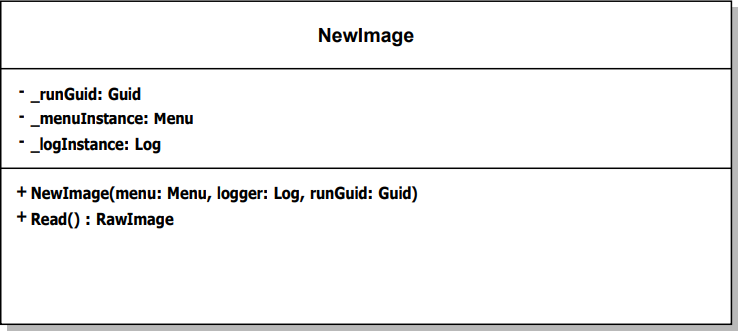
\includegraphics[width=13cm]{images/UML/NewImage.png}}}
    \end{figure}\\

    This is located in the local application and is only responsible for handling the error detection and getting a user input for the path of the image. Once the class is instantiated and the Read function is called it will prompt the user to enter a file path which then goes onto the pre processing class. Also contained within this class is the specific error handling. It looks out for a Preprocessing Exception as well as all other exceptions, this is to allow for more detailed error messages for the user if something goes wrong.\\\bk

    As well as prompting the user to enter a file this is also where it asks the user if they wish to save the process. If they select yes then this class attaches a new MapFile to the result structure. \\
    \bk

    \pagebreak
\paragraph{Pathfinder \textit{(Class)}} \mbox{} \\

    \begin{figure}[H]
        \centering
        \subfloat[\centering Pathfinder Class Diagram]{{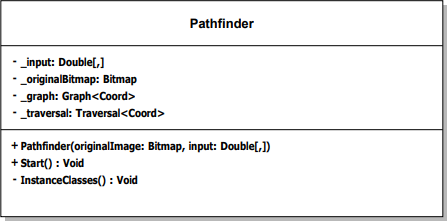
\includegraphics[width=10cm]{images/UML/Pathfinder.png}}}
    \end{figure}\\

    This is located in the front end of the project and is mainly used to keep class coupling to a minimum. Before I implemented operator extensions the conversion to graph was completed here, for now the .ToGraph extension is used to convert the road detected image into a graph. This is done in the InstanceClasses function. Once the classes have been created, a new Windows form instance is created. This is the final stage of the entire program. \\

    \bk

    \pagebreak
\paragraph{Pathfind Image Form \textit{(Windows Form)}} \mbox{} \\

    \begin{figure}[H]
        \centering
        \subfloat[\centering Pathfind Image Form UML Diagram]{{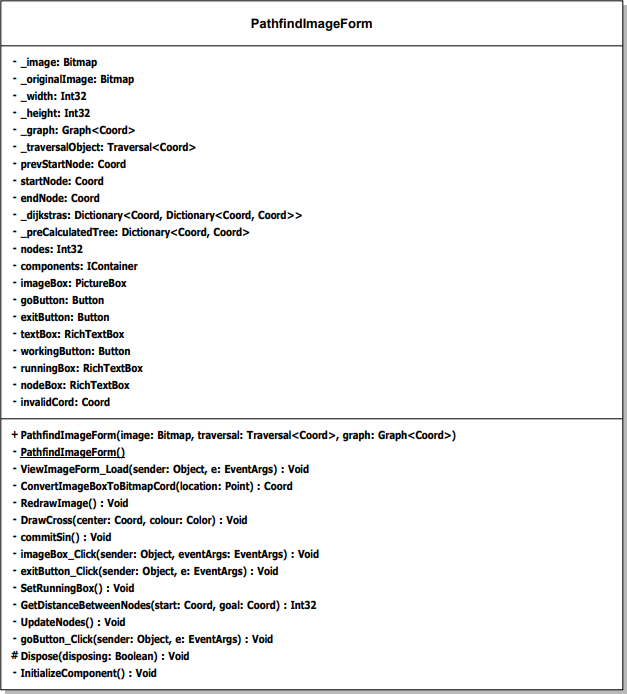
\includegraphics[width=15.5cm]{images/UML/PathfindImageForm.png}}}
    \end{figure}\\

    This is located in the front end of the project. This is the endpoint of the program, all of the processing leads to this point. The form consists of two buttons and a image. Once of the buttons allows the user to exit the program, the other starts the pathfind process. The exit button kills the forms instance and returns to the main menu of the program for the whole process to begin again. \\ \bk

    There are many properties on this class the ones which where created by me and their purposes are as follows:\\

    \begin{itemize}
        \item \_image - This is the image which is shown to the user in the form.
        \item \_originalImage - This is the original image to get round the fact that the old path would be duplicated overlaying multiple paths on-top of each other.
        \item \_width - The width of the image used for bound checking
        \item \_height - The height of the image used for bound checking
        \item \_graph - The graph which is used to traverse the image and therefore draw a path.
        \item \_traversalObject - This is the instantiated class which contains the traversal functions.
        \item \_invalidCoord - A coordinate with values -1 and -1 which is impossible allowing me to detect when not all nodes have been selected.
        \item prevStartNode - The previous start node, used in dijkstra's for working out if the whole algorithm needs to be re-run.
        \item startNode - The start node for any traversal algorithm
        \item endNode - The desired end node for any traversal algorithm
    \end{itemize}\\ \bk

    The way the form gets the user inputs is through a combination of event handlers. When the user left click on the image it sets a new start node and when they right click it sets a new end node. To denote this on the image a red or green cross is placed. If the user has selected for the nodes to bind to the path an algorithm runs over every node and gets the closest one and then draws the node there. \\ \bk

    When it comes down to the pathfinding, the form recalls the settings and runs the selected algorithm. There are some special conditions, if the start node and the end node are the same then the algorithm will not run. If Dijkstra's is selected and a run has been done before and the start node is the same then the algorithm will just re-run the back propagation algorithm and then redraw the path. This is nearly instant, if one of these cases apply then the algorithm is run and the rebuilding of the path is used to find the path the algorithm found. \\ \bk

    The form will have the information of the chosen algorithm on the side above the buttons, this is there to tell the user what is going on at any given point. If dijkstra's is selected then the amount of nodes so far proceeded giving a rough time to completion. \\ 


    \bk

    \pagebreak
\paragraph{Post \textit{(Class)}} \mbox{} \\

    \begin{figure}[H]
        \centering
        \subfloat[\centering Post Class Diagram]{{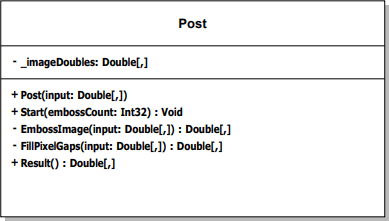
\includegraphics[width=10cm]{images/UML/Post.png}}}
    \end{figure}\\

    This is located in the backend of the project and is responsible for taking the output of the canny edge detection and correcting any errors in it and making it better and fillable for the next stage.
    
    The first method of the of the road result iis only one of to which are available outside of the class, this is of course the Start function. This is used along with a integer to loop over the entire image an apply an embossing kernel then a filling algorithm this filling algorithm is explained in the algorithms section. The integer which is passed in tells the function how many times to perform the operations. If 0 is passed it will just fill the gaps. The way in which it functions when looping is it will call the EmbossImage function and then the FillPixelGaps.\\ \bk

    The result method, in a similar manner to many other classes in this project returns the result of the post processing on the image.\\
    \bk

    \pagebreak
\paragraph{Pre \textit{(Class)}} \mbox{} \\

    \begin{figure}[H]
        \centering
        \subfloat[\centering Pre Class Diagram]{{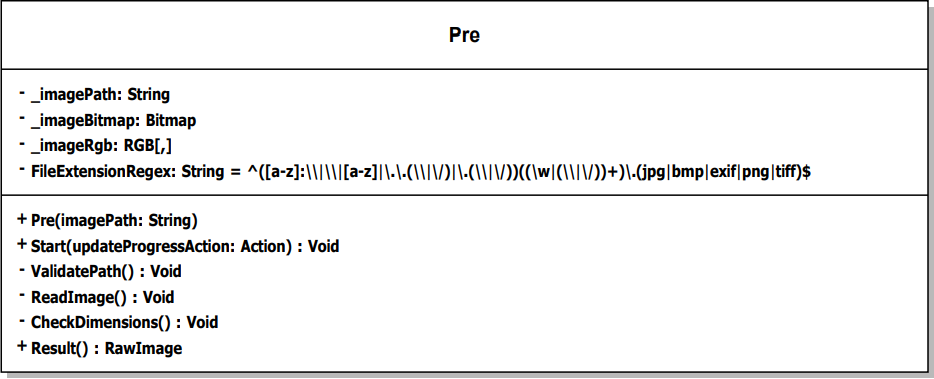
\includegraphics[width=14.5cm]{images/UML/Pre.png}}}
    \end{figure}\\

    This is located in the backend portion of my project, this is responsible for taking in the path a user enters and checking if it is an image, if it is then it reads it in and parses it to a machine understandable state. The most important property on this class is the FileExtensionRegex, this is used to check if the path of the image is correct. As can be seen the program only accepts jpg, bmp, exif, png and tiff image formats. \\ \bk
    
    If the ValidatePath function returns true then the pre processing moves onto the next stage. Once the image has been read into the program using the inbuilt System.Drawing.Bitmap class the data is stripped out from the bitmap and stored in the _imageRGB property. This is to ensure that the program runs efficiently. It turns out that fetching per pixel from a bitmap image is very inefficient and can cause the program to slow down, as well as this Bitmaps are unsafe meaning that they can cause memory issues if mishandled. \\ \bk

    After being read in the image is checked to see if its the right size, if it is not then it is resized to an even amount. The reason that the dimensions of the image have to be even is so that it can be split up into 4 sections with little issues. Once all of this has been completed it is bundled into a structure and awaited to be fetched by the Result function which is called in the main program thread.\\
    \bk

    \pagebreak
\paragraph{Preprocessing Exception \textit{(Exception)}} \mbox{} \\

    \begin{figure}[H]
        \centering
        \subfloat[\centering Preprocessing Exception Class Diagram]{{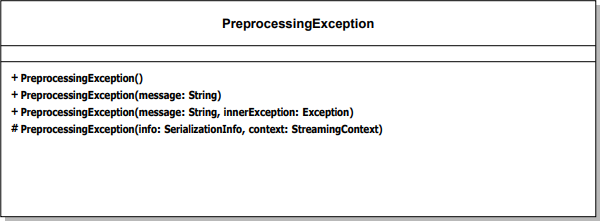
\includegraphics[width=14.5cm]{images/UML/PreprocessingException.png}}}
    \end{figure}\\
    Located in the backend of the project this is a specific exception used to differentiate errors in the front end. This inherits the methods of the base exception class. This is the same as all other custom exception classes. They exist to allow me in the front end to show special error messages.
    \bk

    \pagebreak
\paragraph{Program \textit{(Class)}} \mbox{} \\

    \begin{figure}[H]
        \centering
        \subfloat[\centering Program Class Diagram]{{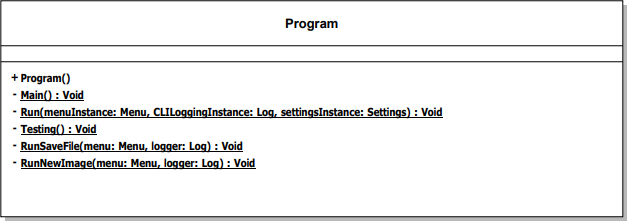
\includegraphics[width=14.5cm]{images/UML/Program.png}}}
    \end{figure}\\

    This is the entry point for the entire application. The Main function is where the program enters and is where the initial setup happens. There is also a testing function shown in this diagram which is not part of the program but was instead used to test various parts of functionality in the testing table. \\ \bk

    The final 3 functions are selected when the user chooses where they wish to go in the program. Run is the function where the program ends into waiting for user input, it will show the user a set of options for them to pick. These include, Run New Image, Run Save File and Settings. If they select settings it will start a settings control instance and allow them to edit said settings. If they select to run a new image the RunNewImage method is invoked and will handel the detection, processing and saving of the new image into a map as explained through out this OOP breakdown. Finally if the user selects the save option RunSaveFile is used, this will prompts the user for a save file, read it in and give the user options for what to do next. This can be seen in the DFD diagrams above.
    \bk

    \pagebreak
\paragraph{Progress Bar \textit{(Class)}} \mbox{} \\

    \begin{figure}[H]
        \centering
        \subfloat[\centering Progress Bar Class Diagram]{{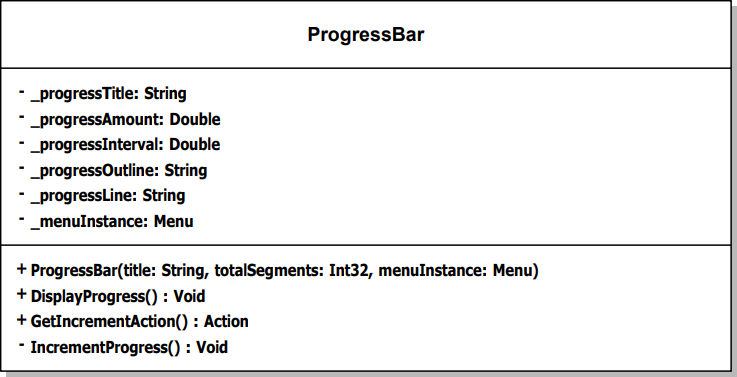
\includegraphics[width=12.5cm]{images/UML/ProgressBar.png}}}
    \end{figure}\\

    The progress bar is very simple and located in the front end of the project. This for me was one of the most important aspects of the program, since from talking to my end user and other possible users of this program, the one thing which they really did not want was the program to just hang and do nothing while they didn't know what was going on. The way which I came to remedy this was through the use of a progress bar. \\ \bk

    The bar fills the user info potion of the screen, the constructor is called with the title, total amount of segments required and a menu instance. The total segments allow the program to calculate how many portions to divide the bar into. Once the program has created a new instance of the progress bar it needs to be displayed on the screen, this is what the DisplayProgress function is for. It draws the outline of the bar only. \\ \bk

    Due to the nature of the progress bar it may be called from separate threads and in the backend where I do not want the front end interacting. In order to get around this Actions are used. When the action is called it adds another segment onto the progress bar in such a way that it does not override the old segments keeping it as fast as possible. The updating of the segments is done here. Once the bar has been completed all that is needed is that the screen be cleared and the instance of the progress bar discarded. \\ 
    \bk

    \pagebreak
\paragraph{Queue \textit{(Class)}} \mbox{} \\

    \begin{figure}[H]
        \centering
        \subfloat[\centering Queue Class Diagram]{{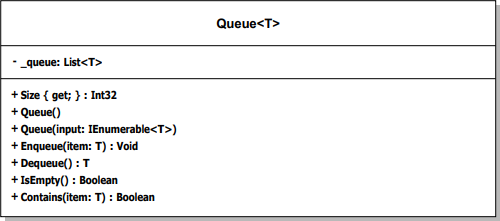
\includegraphics[width=12.5cm]{images/UML/Queue.png}}}
    \end{figure}\\

    This ADT is located in the backend library of my project. The reason which I created my own Queue class is that I needed to be able to directly access parts of it which might not be considered by the inbuilt class. It still contains the same methods as the inbuilt queue:\\ \bk

    \begin{itemize}
        \item Enqueue: Adds an element to the end of the queue.
        \item Dequeue: Removes the element from the front of the queue and returns it.
        \item Peek: Returns the element at the front of the queue without removing it.
        \item Is Empty: Returns a boolean indicating whether the queue is empty or not.
        \item Size: Returns the number of elements in the queue.
        \item Contains: Returns a boolean indicating whether the queue contains an element or not.
    \end{itemize}

    I allowed the queue to be instantiated with a pre existing enumerable, this allows me to create queues with nodes of a graph for example, this is not possible with the queue which was available to me by default. This is used in the traversal class when performing BFS.\\

    \bk

    \pagebreak
\paragraph{Raw Image \textit{(Structure)}} \mbox{} \\

    \begin{figure}[H]
        \centering
        \subfloat[\centering Raw Image Class Diagram]{{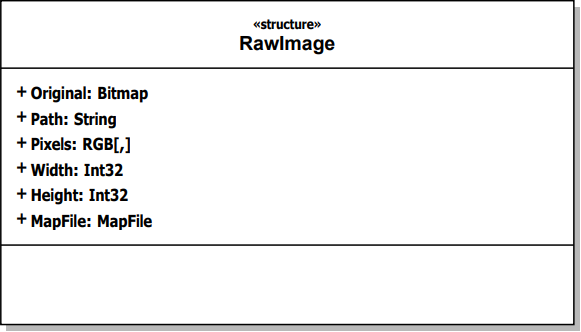
\includegraphics[width=10cm]{images/UML/RawImage.png}}}
    \end{figure}\\

    This is a structure and therefore located in the backend portion of the project. Its function is to move the results of the image about. It contains the original image which was processed, the string representation of the file path as well as the dimensions of said image. These are included to speed up mathematical calculations. It also contains a RGB 2D array which is a more mutable representation of the image. This allows it to be easily converted into other forms and have various algorithms applied to it. Finally a MapFile can be attached to this structure however in the event that no save is selected this will be null to allow the program to see that no save needs to be made.\\

    \bk

    \pagebreak
\paragraph{RGB \textit{(Structure)}} \mbox{} \\

    \begin{figure}[H]
        \centering
        \subfloat[\centering RGB Class Diagram]{{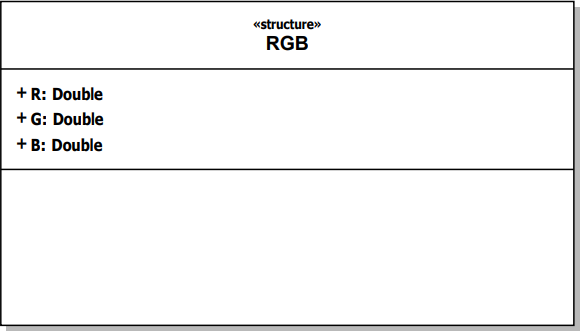
\includegraphics[width=10cm]{images/UML/RGB.png}}}
    \end{figure}\\

    This basic structure is located in the backend library of my final solution. Whilst it does not contain much information this is used in place of the inbuilt Color class due to the limitation that the inbuilt Color class has. It contains just 3 doubles, one for each colour channel. There are overloads involving this class however they are covered by the extensions class so see there for those functions.\\
    \bk

    \pagebreak
\paragraph{Road Detection \textit{(Class)}} \mbox{} \\

    \begin{figure}[H]
        \centering
        \subfloat[\centering Road Detection Class Diagram]{{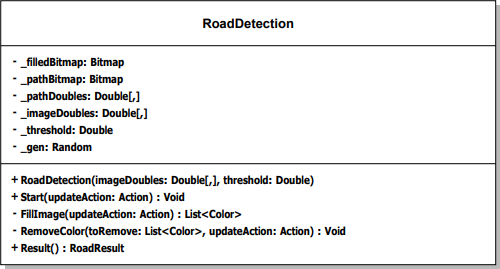
\includegraphics[width=12.5cm]{images/UML/RoadDetection.png}}}
    \end{figure}\\

    This is located in the backend section of my program. Again as with most of my classes in this program it follows the same design of having a Start function which beings the process and a Result function which is called after it has completed and the data returned. The main two processes completed in here are the random colour filling of the canny edge detected image. This functions by generating 3 random integers between 0 and 255, it then uses these to create a Color object. If this has been used before then it regenerates it. this give a possible amount of colours of 255^3 which is 16581375 possibilities. It then performs flood fill with the random colour for each section. This the means every section is unique. After the image has been filled its time to remove the colours which violate the area rules. This is explained in more detail in the area rectification section of the algorithms. \\ \bk

    Once the area rectification has been applied to each section, those which violate the area rules are removed. Once this has been done we now have a final image with the roads on it. Then as one final step all the filled sections are converted to white and the white boarders are removed. Therefore, overall we are just left with a "road no road" map.\\

    \bk

    \pagebreak
\paragraph{Road Result \textit{(Structure)}} \mbox{} \\

    \begin{figure}[H]
        \centering
        \subfloat[\centering Road Result Class Diagram]{{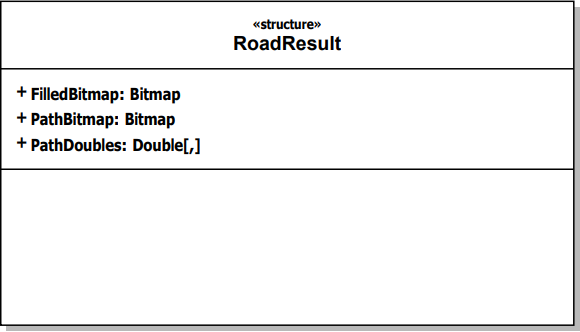
\includegraphics[width=10cm]{images/UML/RoadResult.png}}}
    \end{figure}\\

    This structure is located in the backend portion of the solution, as the name might suggest it is responsible for the result of the road detection. By the stage that this is used the picking out of the roads has occurred and been calculated. The next stage is pathfinding. The filled bitmap is returned so that the user can see how the image was filled and the different section that where picked out. The path bitmap is returned to be stored in the save file if the user requests it. Finally the 2D double array is ued in the pathfinding to tell whether the selected nodes are on the path. It is also used when creating the graph to be routed.\\

    \bk

    \pagebreak
\paragraph{Road Sequence \textit{(Class)}} \mbox{} \\

    \begin{figure}[H]
        \centering
        \subfloat[\centering Road Sequence Class Diagram]{{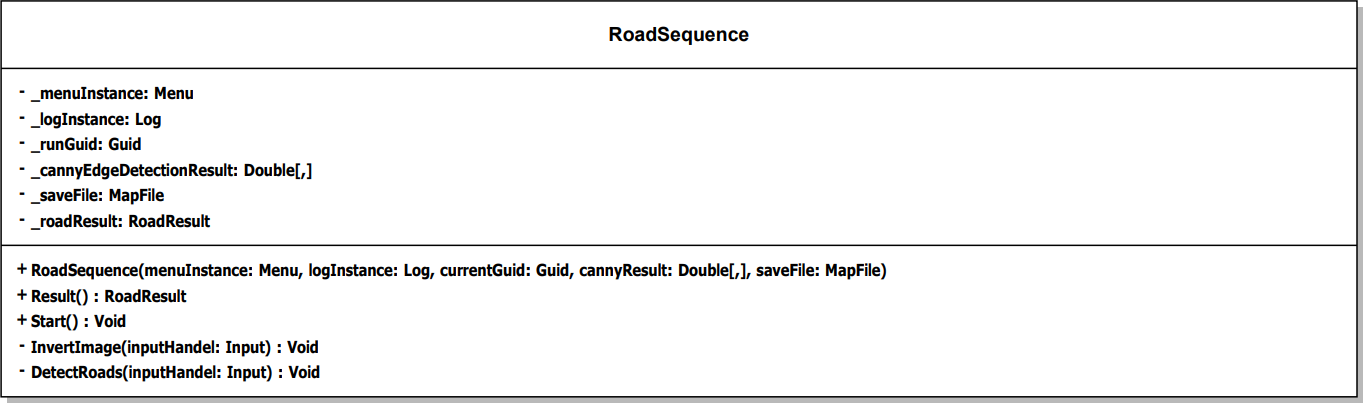
\includegraphics[width=15cm]{images/UML/RoadSequence.png}}}
    \end{figure}\\

    This is located in the front end library of the project. The main two functions here are the InverseImage function and RoadDetection function. Its function is to wrap the backend library calls to ensure that class coupling and code cleanliness is maintained. The inverse image function prompts the use if there are clear roads outlined then the user is asked not to invert the image. Otherwise it is. In this case the save file also needs to be updated to show that the image was inverted. \\ \bk

    Next the RoadDetection function proceeds to create a new instance of the RoadDetection class and start it with a user inputted amount of iterations. The RoadDetection class performs several algorithms as described above an amount of times in accordance with the user inputted value. Once it has completed it will have the Result method called upon it. Once all of this has completed the program moves onto the pathfinding section.\\
    \bk

    
    \pagebreak
\paragraph{Save File \textit{(Class)}} \mbox{} \\

    \begin{figure}[H]
        \centering
        \subfloat[\centering Save File Class Diagram]{{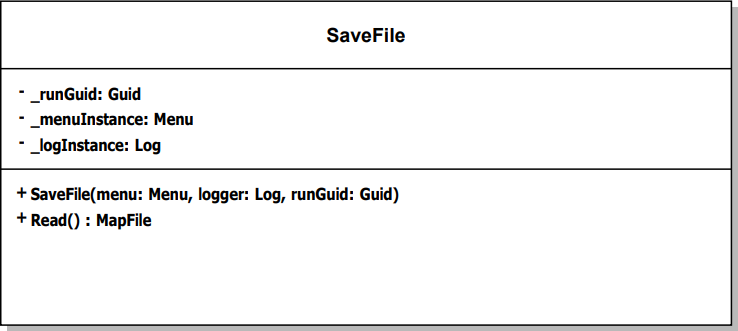
\includegraphics[width=12.5cm]{images/UML/SaveFile.png}}}
    \end{figure}\\

    This is again a very basic wrapper class located in the front end section of the project. This prompts the user to enter the location of a save file and if it exists it fetches it using a MapFile instance. It contains all of the error handling to provide detailed feedback based on the exceptions thrown. It gets the location using the Input GetInput function.\\

    \bk

    
    \pagebreak
\paragraph{Settings \textit{(Class)}} \mbox{} \\

    \begin{figure}[H]
        \centering
        \subfloat[\centering Settings Class Diagram]{{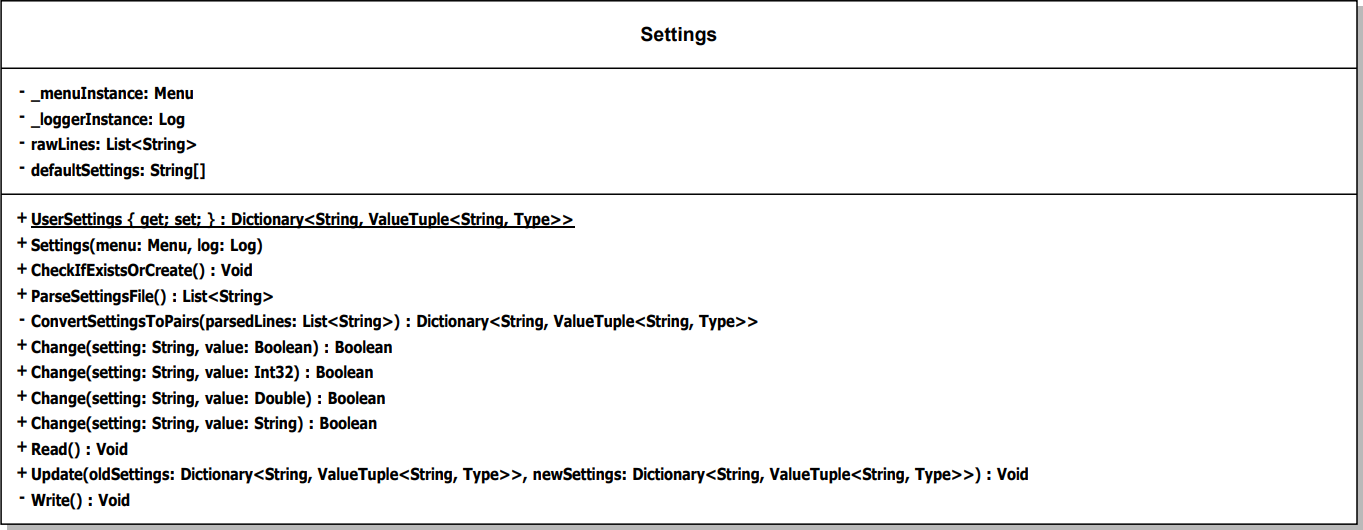
\includegraphics[width=15cm]{images/UML/Settings.png}}}
    \end{figure}\\
    This is located in the frontend portion of the project. This is responsible for handling the settings configuration file itself and the data that comes with it. The main portions of this are to do with parsing the file. Due to the fact that this is not a custom binary file and can be edited by the user in a text document the parsing needs to be bullet proof. \\ \bk

    On creation of the program the settings is not immediately loaded, this is due to the fact that it could be corrupt and we want the program to run at least once. When it is loaded it still will not crash it will throw an error only when the setting was changed and was attempted to be changed. \\ \bk

    The CheckIfExistsOrCreate function is called right at the beginning, this function checks to see if the settings file exists and if it does it reads it into memory and if it does not then it creates the file and reads it into memory. The reading the setting and parsing is done in the ParseSettingsFile function. The way in which the settings are formatting is as follows:\\ \bk

    \begin{pseudocode}
# Manually Edit At Own Risk
# General Settings
detailedLogging=false
forceFormsFront=true

# Pathfinding Settings
convertToMST=false
pathfindingAlgorithm=AStar
snapToGrid=true
endOnFind=false

# Save Settings
shortNames=false
zipOnComplete=false
    \end{pseudocode}\\\bk

    The 4 change functions are used to alter the values of settings and if it is successful the it returns true. When all changing of settings is done the Write method can be invoked. This updates the settings.conf file as well as updating the stored settings in memory. There are various functions that assist with this parsing back into a human form such as ConvertSettingsToPairs.\\\bk

    Update is used to change the old settings to new settings, inside here a sanity check is done to make sure that no extra settings have somehow been included. \\ \bk

    \bk

    \pagebreak
\paragraph{Settings Control \textit{(Class)}} \mbox{} \\

    \begin{figure}[H]
        \centering
        \subfloat[\centering Settings Control Class Diagram]{{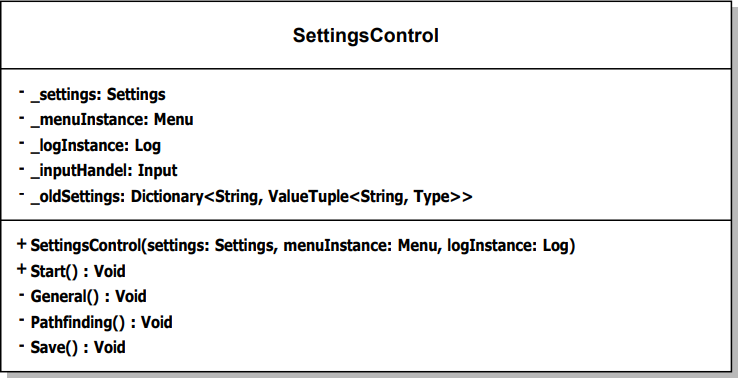
\includegraphics[width=12.5cm]{images/UML/SettingsControl.png}}}
    \end{figure}\\
    This is located in the frontend application of the project, this class is used to allow the user to interact with the settings in a programmatic manner. When this class is created and the Start method is called, this clears the main user section and then displays 3 options to the user. General settings, Pathfinding settings and Save settings. Depending on which of these the user selects the matching General, Pathfinding and Save functions. These allow the user to change these settings and then once exited the settings are updated accordingly. \\ \bk

    This is in essence a abstraction layer on top of the original Settings class. \\
    \bk

    \pagebreak
\paragraph{Settings Exception \textit{(Exception)}} \mbox{} \\

    \begin{figure}[H]
        \centering
        \subfloat[\centering Settings Exception Class Diagram]{{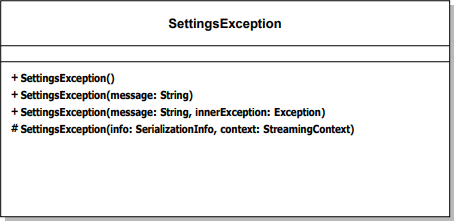
\includegraphics[width=10cm]{images/UML/SettingsException.png}}}
    \end{figure}\\
    Located in the backend of the project this is a specific exception used to differentiate errors in the front end. This inherits the methods of the base exception class. This is the same as all other custom exception classes. They exist to allow me in the front end to show special error messages.
    \bk

    \pagebreak
\paragraph{Stack \textit{(Class)}} \mbox{} \\

    \begin{figure}[H]
        \centering
        \subfloat[\centering Stack Class Diagram]{{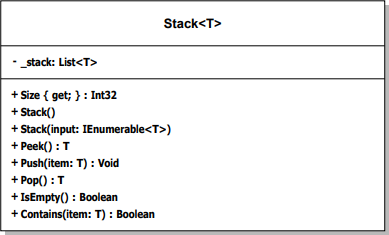
\includegraphics[width=8cm]{images/UML/Stack.png}}}
    \end{figure}\\

    This is an ADT located in the backend of my project. In a similar vain to the Queue class I needed to be able to durectly acess parts which where not available in the default stack class. It contains the following:

    \begin{itemize}
        \item Push: Adds an element to the end of the stack.
        \item Pop: Removes the element from the end of the stack and returns it.
        \item Peek: Returns the element at the end of the stack without removing it.
        \item Is Empty: Returns a boolean indicating whether the stack is empty or not.
        \item Size: Returns the number of elements in the stack.
        \item Contains: Returns a boolean indicating whether the stack contains an element or not.
    \end{itemize}

    There is a similar modification allowing for any I enumerable to be passed to instantiate the Stack. With the Queue as well it can be seen from the class diagram that all of the methods are generic meaning that this will work with any data type allowing the graph and subsequent traversal to work in all cases.\\

    \bk

    \pagebreak
\paragraph{Structures \textit{(Class)}} \mbox{} \\

    \begin{figure}[H]
        \centering
        \subfloat[\centering Structures Class Diagram]{{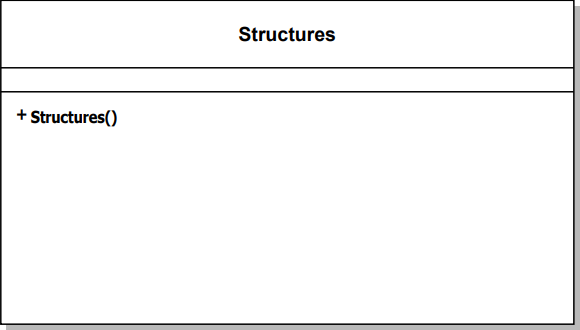
\includegraphics[width=8cm]{images/UML/Structures.png}}}
    \end{figure}\\

    This is located in the backend of the project, this is due to the fact that all it contains is the structures which can be seen written out below. Each of them contains public properties which can then be used in the program to move large amounts of data around without the need for massive tuples.

    \begin{figure}[H]
        \centering
        \subfloat[\centering Structures Class Diagram]{{\includegraphics[width=17.2cm]{images/UML/Backend.png}}}
    \end{figure}\\


    \bk

    \pagebreak
\paragraph{Sync Edge Detection \textit{(Class)}} \mbox{} \\

    \begin{figure}[H]
        \centering
        \subfloat[\centering Sync Edge Detection Class Diagram]{{\includegraphics[width=12.5cm]{images/UML/SyncEdgeDetection.png}}}
    \end{figure}\\

    This is located in the local application section of the solution. In essence all that this class does is to provide a layer of abstraction on top of the edge detection. The first thing that occurs in this class once it is instantiated is that it asks the user to enter the initial paraders for whatever stage is first, this happens to be conversion to greyscale. It will then confirm the parameters with the user, if the user says yes then the program performs the precess. After it has performed the process it asks the user if this was the output they where expecting. If it is not then they can change the parameters and go again. This happens with all the stages of canny edge detection. \\ \bk

    The difference between this and the async version is that the async version runs all at once and there is no chance to redo steps. Whereas here the outputs are shown the user in the View Image Form after ever step. The result of the SyncEdgeDetection class is fetched the same way as the async version. This is the point of the IHandler interface. \\ \bk

    Not all of the stages of the single threaded version are available to be tweaked and these do run similarly to the async version with threading. \\
    \bk


    \pagebreak
\paragraph{Text Wall \textit{(Class)}} \mbox{} \\

    \begin{figure}[H]
        \centering
        \subfloat[\centering Text Wall Class Diagram]{{\includegraphics[width=12.5cm]{images/UML/TextWall.png}}}
    \end{figure}\\

    This is located in the front end section of the program. It is used to send blocks of text which may be used more than once to keep the code clean and editable. The functions in here are self explanatory and send messages to the user they are not integral to the function of the program and are just separated for ease of use. \\ 

    \bk

    \pagebreak
\paragraph{Threshold Pixel \textit{(Structure)}} \mbox{} \\

    \begin{figure}[H]
        \centering
        \subfloat[\centering Threshold Pixel Class Diagram]{{\includegraphics[width=12.5cm]{images/UML/ThresholdPixel.png}}}
    \end{figure}\\

    This is a structure and located in the backend library of the project. It is only used in the edge detection section however it is vital in the final hysteresis stage. It allows the program to tell if a pixel needs to be made strong or not. This structure therefore contains the greyscale value of the pixel it represents as a double and whether it is considered strong or not. This is represented by a boolean. The general way that this is implemented is in a 2D array removing the need to have coordinates stored in the structure itself.

    \bk

    \pagebreak
\paragraph{Traversal \textit{(Class)}} \mbox{} \\

    \begin{figure}[H]
        \centering
        \subfloat[\centering Traversal Class Diagram]{{\includegraphics[width=12.5cm]{images/UML/Traversal.png}}}
    \end{figure}\\

    This is the class which is responsible for the functionality relating to the pathfinding of the map. This is located in the backend library of the project. It contains 4 different traversal and searching algorithms each of which will be explained below. \\ \bk

    \textbf{BFS / DFS} \\
    I have chosen to combine these two together due to the fact that they are essentially identical bar from the fact that one of them uses a stack and the other a queue. The pseudocode for each is below:\\
    \begin{pseudocode}
// DFS
procedure DFS_iterative(G, v) is
let S be a stack
S.push(v)
while S is not empty do
    v = S.pop()
    if v is not labelled as discovered then
        label v as discovered
        for all edges from v to w in G.adjacentEdges(v) do 
            S.push(w)

// BFS
procedure BFS_iterative(G, v) is
let S be a queue
S.push(v)
while S is not empty do
    v = S.pop()
    if v is not labelled as discovered then
        label v as discovered
        for all edges from v to w in G.adjacentEdges(v) do 
            S.push(w)
    \end{pseudocode} \\ \BK

    \textbf{Dijkstra's} \\
    \begin{pseudocode}
function Dijkstra(Graph, source):
    dist[source] ← 0                           // Initialization
    create vertex priority queue Q
    for each vertex v in Graph.Vertices:
        if v ≠ source
            dist[v] ← INFINITY                 // Unknown distance from source to v
            prev[v] ← UNDEFINED                // Predecessor of v

        Q.add_with_priority(v, dist[v])


    while Q is not empty:                      // The main loop
        u ← Q.extract_min()                    // Remove and return best vertex
        for each neighbor v of u:              // Go through all v neighbors of u
            alt ← dist[u] + Graph.Edges(u, v)
            if alt < dist[v]:
                dist[v] ← alt
                prev[v] ← u
                Q.decrease_priority(v, alt)

    return dist, prev
    \end{pseudocode} \\ \BK

    \textbf{A* Search} \\
    \begin{pseudocode}
function reconstruct_path(cameFrom, current)
    total_path := {current}
    while current in cameFrom.Keys:
        current := cameFrom[current]
        total_path.prepend(current)
    return total_path

// A* finds a path from start to goal.
// h is the heuristic function. h(n) estimates the cost to reach goal from node n.
function A_Star(start, goal, h)
    // The set of discovered nodes that may need to be (re-)expanded.
    // Initially, only the start node is known.
    // This is usually implemented as a min-heap or priority queue rather than a hash-set.
    openSet := {start}

    // For node n, cameFrom[n] is the node immediately preceding it on the cheapest path from start
    // to n currently known.
    cameFrom := an empty map

    // For node n, gScore[n] is the cost of the cheapest path from start to n currently known.
    gScore := map with default value of Infinity
    gScore[start] := 0

    // For node n, fScore[n] := gScore[n] + h(n). fScore[n] represents our current best guess as to
    // how cheap a path could be from start to finish if it goes through n.
    fScore := map with default value of Infinity
    fScore[start] := h(start)

    while openSet is not empty
        // This operation can occur in O(Log(N)) time if openSet is a min-heap or a priority queue
        current := the node in openSet having the lowest fScore[] value
        if current = goal
            return reconstruct_path(cameFrom, current)

        openSet.Remove(current)
        for each neighbor of current
            // d(current,neighbor) is the weight of the edge from current to neighbor
            // tentative_gScore is the distance from start to the neighbor through current
            tentative_gScore := gScore[current] + d(current, neighbor)
            if tentative_gScore < gScore[neighbor]
                // This path to neighbor is better than any previous one. Record it!
                cameFrom[neighbor] := current
                gScore[neighbor] := tentative_gScore
                fScore[neighbor] := tentative_gScore + h(neighbor)
                if neighbor not in openSet
                    openSet.add(neighbor)

    // Open set is empty but goal was never reached
    return failure
    \end{pseudocode} \\ \BK

    This is all that is contained within the traversal algorithm, the only properties on this class is te graph which is having the algorithms applied to it. I chose to instantiate the class with the graph instead of passing it in as a reference to keep the classes couples and to avoid data from getting altered unexpectedly.
    \bk

    \pagebreak
\paragraph{Utility \textit{(Class)}} \mbox{} \\

    \begin{figure}[H]
        \centering
        \subfloat[\centering Utility Class Diagram]{{\includegraphics[width=14cm]{images/UML/Utility.png}}}
    \end{figure}\\

    This is located in the backend library of this solution. The main function of this class is to supplement the various other classes and algorithms, therefore the easiest way to describe the functions is going through each function in tern. \\ \bk

    \textbf{GaussianDistribution} \\ \bk
    This function is responsible for generating the gaussian values for the gaussian kernel. It returns the result of a 2D gaussian distribution calculation.\\\bk


    \textbf{Bound} \\ \bk
    This take 3 values, the upper bound, the lower bound and the value to be bounded. If the value is outside the bounds then it is set to the closest bound. For example if the lower bound is 0 and upper bound is 100 and 150 is passed in. The bounded value is 100.\\\bk

    \textbf{TryBound} \\ \bk
    This performs the exact same as above except it returns true if the value provided was within the bounds.\\\bk

    \textbf{RadianToDegree} \\ \bk
    Converts Radians to Degrees through \frac{180}{2\pi}\\\bk
    \textbf{DegreeToRadian} \\ \bk
    Converts Degrees to Radians through \frac{2\pi}{180}\\\bk

    \textbf{MapRadiansToPixel} \\ \bk
    This takes in a double value which is a radian measurement, converts it to degrees then bounds it to between 0 and 255.\\\bk
    \textbf{CombineBitmap} \\ \bk
    This takes two images in the form of bitmaps and combines B on top of A. Returns a reference to a new bitmap (not A or B).\\\bk

    \textbf{SplitImage} \\ \bk
    This takes an input of a 2D array of RGB structures. It then calculates the size of 4 quadrants, and returns the 4 quadrants of each image, this then goes on to be used to speed up the edge detection.\\\bk
    
    \textbf{CombineQuadrants} \\ \bk
    This combines 4 quadrants into one large sector.\\\bk
    \textbf{InverseImage} \\ \bk
    This takes in a 2D double array of values of either 0 or 255 and then flips them. If it was 0 it is now 255 and vice versa, in essence it inverts all the pixels / doubles in the image.\\\bk

    \textbf{RebuildPath} \\ \bk
    This takes the output from any one of the graph traversal algorithms and uses the dictionary it generated to form a path given a generic end node. If the node does not exist it returns an empty array.\\\bk
    
    \textbf{IsYes} \\ \bk
    Takes a text input and returns true if it deems the text was a confirmation and false otherwise.\\\bk

    \textbf{GetRed} \\ \bk
    Gets the red value of a Color object.\\\bk
    \textbf{GetGreen} \\ \bk
    Gets the green value of a Color object.\\\bk
    \textbf{GetBlue}
    Gets the blue value of a Color object.\\\bk
    \textbf{GetAverage} \\ \bk
    Gets the average of all colour channels, it does this by adding them all together then dividing by 3.\\\bk
    \textbf{GetIndustryAverage} \\ \bk
    This applies the industry average ratios to the pixel to get an average approximation of a greyscale pixel.\\\bk
    \textbf{GetIfExists} \\ \bk
    If the Colour object has any colour whatsoever it will return 255.\\\bk
    \textbf{GetDistanceBetweenNodes} \\ \bk
    Gets the pythagorean distance between two coordinates.\\

    \bk

    \pagebreak
\paragraph{View Image Form \textit{(Windows Form)}} \mbox{} \\

    \begin{figure}[H]
        \centering
        \subfloat[\centering View Image Form UML Diagram]{{\includegraphics[width=11cm]{images/UML/ViewImageForm.png}}}
    \end{figure}\\

    This is located in the front end of the program and is responsible for showing the image to the user. This is all that the form does and has the image on the left and the continue button on the right. Inside the form is code to dynamically resize the elements of the form to fit the screen. The only function written by me is the nextButton which closes the form and resumes the program.

    \BK

    \subsection{File Structure}
    \subsubsection{Program Files}
    I have taken the decision of splitting my project into a front end and a back end. This came from the interview talking to my end user. They felt that having multiple different ways of interacting with the program. In order to do this I will separate the front end and the back end processing. This is also considered best practice when writing software since it keeps it maintainable. \\ \bk
    
    One of the requirements if I am going to follow this is that there are no user input calls made in the back end portion of the code. However sometimes I may want the user to be kept update as to what is going on in the program and give them a rough estimation of how long is lest, to do this I will employ the use of actions. With actions this means that should I want to extend this in the future to use razor pages for example this can be done with minimal amounts of effort. \\ \bk

    Contained within the front section of the program in this case will be all of the console UI and various classes which will interact with the backend. The one slight issue with this is that the program will then require the DLL of the backend to function which would make the program more complicated to just move to another computer. To get around this I will be using ILmerge and the script below:

    \begin{pseudocode}
C:\\Users\\ruben\\.nuget\\packages\\ilmerge\\3.0.41\\tools\\net452\\ILMerge.exe 
    /out:RubensPirieNEA.exe 
    ..\\bin\\Release\\LocalApp.exe 
    ..\\bin\\Release\\BackendLib.dll
    \end{pseudocode}

    This allows the program to be executed as one single .exe file making it easy of the user to use.\\ 

    \bk

    \subsubsection{Generated Files}
    When the program is run there will need to be certain directories created in order to store the outputs of the files. The requirement for this will need to be every time the program runs it will check to see if the directories and files exist, if they do not then it will create them. If they do then it will not create one or override the existing files. \\ \bk

    The directory structure will be as follows:
    \begin{pseudocode}
    .
    └── Program/
        ├── saves/
        │   └── <run-id>
        ├── runs/
        │   └── <run-id>/
        │       └── image(s).png
        ├── logs/
        │   ├── <run-id>.log
        │   └── master.log
        └── settings.conf
    \end{pseudocode}

    The main reason which I am going with this structure is that I feel it makes navigating the program easy and intuitive. Since the logs of what are happening will be stored in the log directory, run files in the runs directory and so on and so forth. \\ \bk

    The reason as to why I have chosen to move the settings file out to the root of the program files is that this is going to be the thing that needs to be most quickly accessed by the user and therefore should be easy to get too. I did consider using a database for the settings of the project however have decided against it due to the fact that it would add extra overhead which is not needed. \\ \bk

    I did consider using some other form of storing the user outputs from the program, however as one of my extension objectives is to compress all of the outputs into one format which can be drag and dropped I felt that files where the easiest way to go. The custom binary file is also compatible with being windows zipped so I saw no issues with using standard binary and text files in this case. \\ \bk

    \BK

    \subsection{Algorithms}

    \subsubsection{Edge Detection}
    This has been explained in detail in the class breakdown and analysis sections of this report. Here I will explain the general idea behind edge detection as a whole and what method it plays here. \\ \bk

    The purpose of edge detection is to allow an application to pick out the edges of a common example of this is in parcel courier services where when a parcel is being shipped they will need to be able to find the exact dimensions of the parcel but cannot afford to have someone there to measure every one. In this case edge detection can be used in order to find the outline and therefore allow it to be processed. The relevance of this to my program is that I need to be able to pick out, on a given image, where the roads are. This I feel is a perfect application of edge detection since I will be picking out roads which are characterised by edges on an image. \\ \bk

    There are several different methods of edge detection, the ones which I came across during my research are all examples of searching. Examples of the methods I came across are, Canny (the method I chose), Kovalevsky which takes a rather different approach to Canny where this one uses the second differential of regions in the image to work iut where there are changes in intensity and finally Sobel detection. This is somewhat incorporated into Canny edge detection however the theory behind this is purley mathematical. It involve taking remade matrices and multiplying the image with them. \\ \bk

    The advantage to Canny edge detection is that it has two major advantages:
    \begin{itemize}
        \item High Quality Maps: The way in which the image is processed allows it to preserve the resolution as it flows through the various steps. I want to be able to keep the image as high quality as possible since this is presented to a user and not being used in a machine learning environment.
        \item Accuracy: This method in particular with the first step of the Gaussian filtering, allows the inputs to be noisy, such as a photographed image. This means that I don't have to worry about de-noising the image first. 
    \end{itemize}

    \bk

    \subsubsection{Refinement Algorithm (Custom)}
    This is part of the processing the map into a a computer recognisable form. The stage after this will be filling the image. In order to do this the program must have a closed shape in which it can fill. In order to do this I needed to take the output of the edge detection and make sure that all of the roads where enclosed. \\ \bk

    I have been unable to find a suitable existing algorithm to complete this for me. There are several different types of filling algorithm which will be explained soon. What I did come across in my research is that there are many different types of image kernel and how they can be used to alter image properties. One useful one which I came across was was the embossing kernel. This goes over the images and essentially "bolds" all of the lines in the image. \\ \bk

    With these "bolded lines" it can cause gaps which previously existed to be filled. However there is one final issue which is where the lines have been connected there are intermittent black pixels which haven't been fixed by the embossing kernel. In order to remedy this I will employ a similar method as the hysteresis algorithm in Canny edge detection. \\ \bk
    
    The solution I have come up with is to run over every pixel in the edge map. If there are more than a set number of white "strong" pixels around a black pixel then the black will be replaced with white. What this accomplishes is a "filling" the black pot holes. Overall this does not accomplish much however it means that if an image needs more than one pass of this "fortification" algorithm then this makes the result more reliable in the long run. \\ \bk

    I have also decided that this will need to have the option of being run more than once. I found that during the testing if there where large gaps then the embossing would need to occurs more than once.\\
    \bk

    \subsubsection{Flood Fill}
    This is an algorithm as old as time, I decided to go with th 8 direction flood fill. The premise behind the flood filling algorithm is to start from a seed point in the image and then spread the fill color to all connected pixels in the same region. The algorithm uses a queue to store the pixels that need to be filled, and it works by visiting each pixel in the queue, checking its 8 neighbouring pixels, and adding any unvisited pixels that belong to the same region to the queue. This process continues until all pixels in the region have been visited and filled. \\ \bk

    The algorithm can be implemented in a variety of ways, and it is often used as a building block for more complex image processing, as is being used in this case, algorithms, such as object recognition, image segmentation, and feature extraction. It is also commonly used in video games and user interface design to fill shapes and create smooth animations. \\ \bk

    In my version the other advantage to using the flood fill colours is that it can be shown to the user to clearly outline where the regions where which would allow them to change the thresholds and behaviour of the filling algorithm. Certain things that can be changed are the method of storing the pixels. Either in a queue of a stack. \\ 
    \bk

    \subsubsection{Area Rectification (Custom)}
    This came about due to an issue with the flood filling, the issue with the flood fill is that it fills every single area that there is in the chance that the user will pathfind within a pond marked on the map for example. The solution which I have arrived to to solve this is to take the two extremes of every filled area. \\ \bk

    Using these two extremes we can calculate the square boundary of the filled area.

    $$
        (X_{max} - X_{min}) * (Y_{max} - Y_{min}) = \text{Square Area} 
    $$

    \\ \bk

    With this area we can take the actual filled area of the shape and work out the ratio of one to the other by doing

    $$
        \frac{\text{Actual Area}}{\text{Calculated Area}} = \text{Area Ratio}
    $$
    \\ \bk

    The user will then enter a ratio and if the ratio is greater than the calculated ratio then the area us rejected as not a road. The reason that this works is roads are characteristic's long and winding which means that they will have a small ratio making it easy to single them out. The one downside is that this can produce false positives if there is a thick straight road however in testing this did not seem to be an issue. \\


    \bk

    \subsubsection{Graph Conversion (Custom)}
    This is not an algorithm as such but more of a method to complete a goal. Once the image has been processed to the fullest degree, this is after the road detection and area rectification has taken place.  \\ \bk

    The way that this algorithm functions is that it takes the corrected filled image, it will pass over the entire image converting all "non white" pixels to white and keeping black ones black. After it has done this the program will iterate over all of the pixels in the image and if it is white it will take all of the neighbors and add a connection. \\ \bk

    As an optimisation step I took the decision to only add nodes to the graph which "exist", this cuts down on the nodes in the image drastically. This is because without making this optimisation the amount of neighbors nodes are always 8 which causes the program complexity to drastically increase. Therefore I am making the decision to remove all of those nodes from the graph in the first place. \\ \bk

    The identifier of the nodes will be a Coordinate object which contains the X and Y. These are the references which are stored as the node's children which can then be used to edit the final image to show the user the path.
    \bk

    \subsubsection{Dijkstra's Search Algorithm}
    Dijkstra's search algorithm is a graph search algorithm that is commonly used to find the shortest path between two nodes in a graph. It was first proposed by the Dutch computer scientist Edsger W. Dijkstra in 1956, and it is widely used in computer science, especially in the fields of computer networking, transportation systems, and geographic information systems (similar to my program here). \\ \bk

    The algorithm works by maintaining a priority queue of nodes that have been visited and continually updating the distance to the nearest unvisited node until the destination node has been reached. The algorithm operates as follows:\\

    \begin{itemize}
    \item Start at the source node and set the distance to the source node to zero.

    \item Visit the neighbors of the current node and update their distances based on the distance to the current node and the edge weight between the current node and the neighbors.

    \item Choose the node with the smallest distance as the next node to visit, and mark it as visited. Repeat the process until the destination node has been reached or all nodes have been visited.
    \end{itemize}

    Dijkstra's algorithm is guaranteed to find the shortest path between two nodes in a graph if there are no negative edge weights. The algorithm is efficient and can be implemented in a variety of programming languages, including C#.\\ \bk

    In this map processing project, Dijkstra's algorithm can be used to find the shortest path between two points on a map, which can be useful for navigation, route planning, and other applications. The algorithm can be adapted to work with different types of maps, such as road networks or public transportation systems, by representing the map as a graph and defining the edge weights between nodes based on the specific requirements of this application. \\ \bk

    As I mentioned really usefully for this application because if I could expand the application to work out the weights of different roads based on width. \\ 
    \bk
    
    \subsubsection{A-Star Search Algorithm}
    A* is a graph search algorithm that is commonly used to find the shortest path between two nodes in a graph. It was first proposed by Peter Hart, Nils Nilsson, and Bertram Raphael in 1968 and is considered an extension of Dijkstra's algorithm. \\ \bk

    Like Dijkstra's algorithm, A* operates by maintaining a priority queue of nodes that have been visited, and it continually updates the distance to the nearest unvisited node until the destination node has been reached. The key difference between A* and Dijkstra's is that A* incorporates a heuristic function to estimate the remaining distance from a node to the destination node. This heuristic function allows A* to prioritize nodes that are likely to be closer to the destination node, making it more efficient than Dijkstra's algorithm in many cases. \\ \bk

    The algorithm operates as follows:
    \begin{itemize}
        \item Start at the source node and set the distance to the source node to zero.
        \item Visit the neighbors of the current node and update their distances based on the distance to the current node, the edge weight between the current node and the neighbors, and the estimated remaining distance to the destination node.
        \item Choose the node with the smallest estimated total distance (the sum of the distance to the current node and the estimated remaining distance to the destination node) as the next node to visit, and mark it as visited. Repeat the process until the destination node has been reached or all nodes have been visited.
    \end{itemize}

    A* is often used in computer science and engineering applications that require finding the shortest path between two nodes in a graph, such as computer graphics, video game development, robotics, and artificial intelligence. In this map processing project, A* can be used to find the shortest path between two points on a map, taking into account factors such as road conditions, traffic, and elevation, to provide an optimal route for navigation and route planning which adapts to given conditions. \\ \bk

    Then overriding main reason which I am choosing to go with a validation of A* with cartesian distance is that it is significantly faster and more efficient than Dijkstra's. Although Dijkstra has the advantage of post routing meaning that as long as the start node is the same the route can be found instantly. 
    \bk

    \subsubsection{Binary Heap Min Priority Queue}
    A binary heap is a type of data structure that can be used to implement a priority queue, where elements are kept in order based on their priority. A binary heap can be either a min-heap or a max-heap, depending on whether the smallest or largest element is considered to have the highest priority. In a min-heap, the parent node of the heap has a value that is less than or equal to the values of its children.\\ \bk

    A binary heap is implemented as a complete binary tree, where all levels of the tree are filled except possibly the last one, which is filled from left to right. In a min-heap, the smallest element is stored at the root of the tree, and the two children of a node with a smaller value are stored in the left and right child nodes of that node.\\ \bk
    
    To implement a min-priority queue using a binary heap, we can use the following operations;\\ \bk

    Insertion: To insert an element into the binary heap, it is added to the next available position in the last level of the tree, and then "bubbled up" the tree by swapping it with its parent until the min-heap property is restored.\\ \bk
    
    Extraction of minimum element: To extract the minimum element from the binary heap, we remove the root node and replace it with the last element in the tree. The new root node is then "sunk down" the tree by swapping it with its smaller child until the min-heap property is restored.\\ \bk
    
    Decrease key: To decrease the priority of an element in the binary heap, we first find the element and update its value, and then "bubble up" the node by swapping it with its parent until the min-heap property is restored.\\ \bk
    
    Binary heaps are used in many algorithms, such as Dijkstra's shortest path algorithm and the A* algorithm which happen to be the exact algorithms I am using, because they have the property of being able to efficiently maintain a priority queue in a sorted order. They have a time complexity of O(log n) for inserting and extracting elements, which makes them a fast and efficient data structure for implementing priority queues, keeping the delay of processing low.\\ \bk

    \bk
\end{FlushLeft}